\documentclass[aspectratio=169,10pt,xcolor=pdflatex,dvipsnames,table]{beamer}
\usepackage{newcent}
\usepackage[utf8]{inputenc}
\usepackage[czech]{babel}
\usepackage{hyperref}
\usepackage{amsthm}
\usepackage{amssymb}
\usepackage{amsmath}
\usepackage{array}
\usepackage{stmaryrd}
\usepackage{graphicx}
\usepackage{tabularx}
\usepackage{listings}
\usepackage{fancyvrb}
\usepackage{minted}
\usepackage{multicol}
%\usepackage{packages/beamerthemeFIT}

\makeatletter
  \def\beamer@calltheme#1#2#3{%
    \def\beamer@themelist{#2}
    \@for\beamer@themename:=\beamer@themelist\do
    {\usepackage[{#1}]{\beamer@themelocation/#3\beamer@themename}}}

  \def\usefolder#1{
    \def\beamer@themelocation{#1}
  }
  \def\beamer@themelocation{}

\usefolder{packages}
\usetheme{FIT}



\title[OpenGL]{PGR - Shadows, procedural generation / Stíny, procedurální generování}

\author[]{Tomáš Milet}

\institute[]{Brno University of Technology, Faculty of Information Technology\\
Bo\v{z}et\v{e}chova 1/2. 612 66 Brno - Kr\'alovo Pole\\
imilet@fit.vutbr.cz}

\date{\today}

\begin{document}

\frame[plain]{\titlepage}

\definecolor{bg}{rgb}{0.95,0.95,0.95}

\setbeamercolor{background canvas}{bg=fitblue}
\begin{frame}
\frametitle{Shadows / Stíny}
\begin{center}
\Huge {\color{white}Shadows / Stíny}
\end{center}
\end{frame}
\setbeamercolor{background canvas}{bg=white}

\begin{frame}\frametitle{Why do we need shadows? / Proč potřebujeme stíny?}
  \begin{figure}[h]
    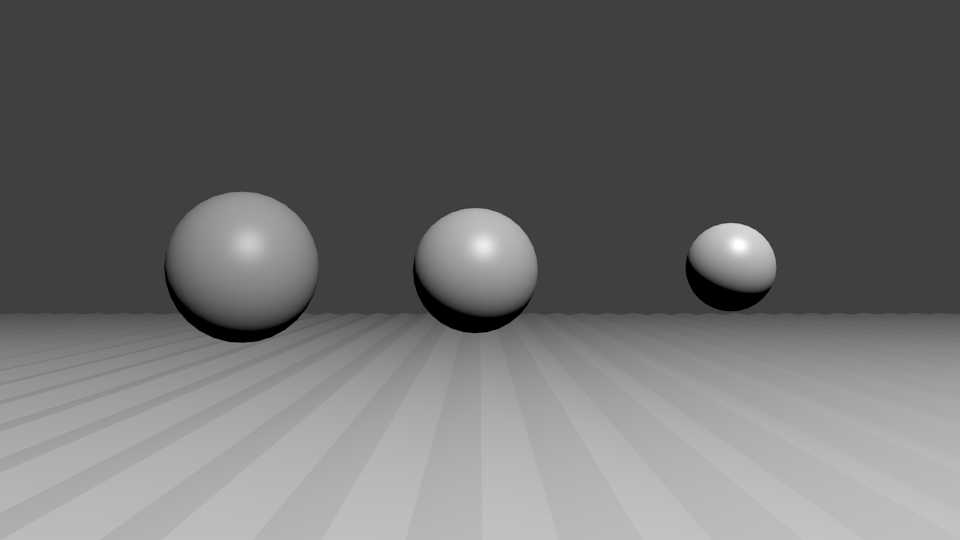
\includegraphics[width=11.5cm,keepaspectratio]{pics/shadows/whyShadows/noShadows}
  \end{figure}
\end{frame}

\begin{frame}\frametitle{Why do we need shadows? / Proč potřebujeme stíny?}
  \begin{figure}[h]
    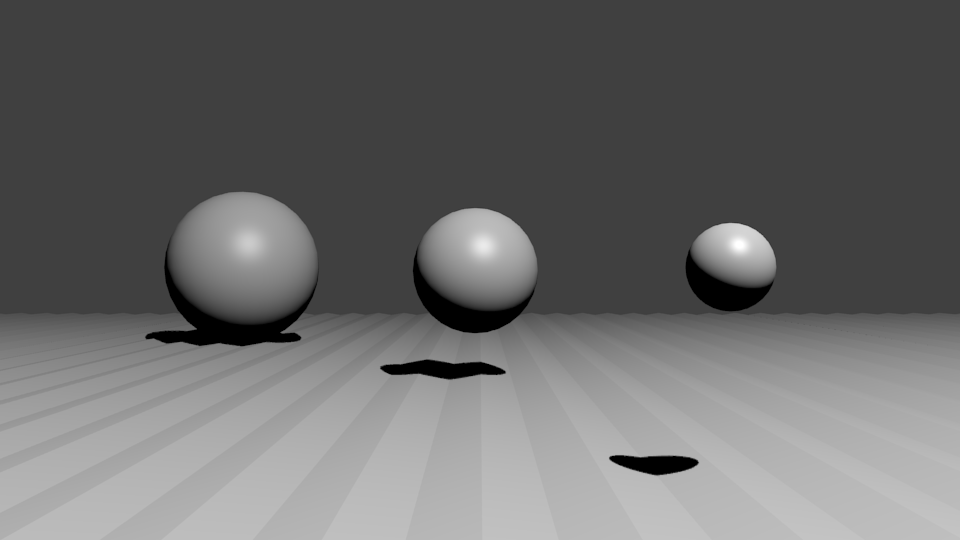
\includegraphics[width=11.5cm,keepaspectratio]{pics/shadows/whyShadows/shadows}
  \end{figure}
\end{frame}

\begin{frame}\frametitle{Why do we need shadows? / Proč potřebujeme stíny?}
  \begin{figure}[h]
    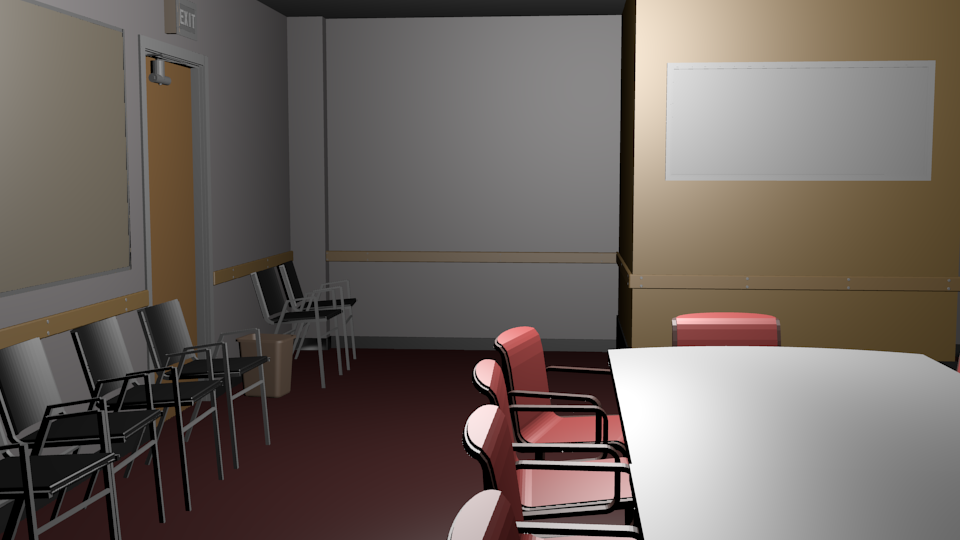
\includegraphics[width=11.5cm,keepaspectratio]{pics/shadows/whyShadows/conferenceNoShadows}
  \end{figure}
\end{frame}

\begin{frame}\frametitle{Why do we need shadows? / Proč potřebujeme stíny?}\scriptsize
  \begin{itemize}
    \item Shadows help us to comprehend 3D structure of a scene.
    \item Mutual location of objects.
  \end{itemize}
  \begin{itemize}
    \item Stíny pomáhají pochopit 3D scénu.
    \item Vzájemné polohy mezi objekty.
  \end{itemize}
  \begin{figure}[h]
    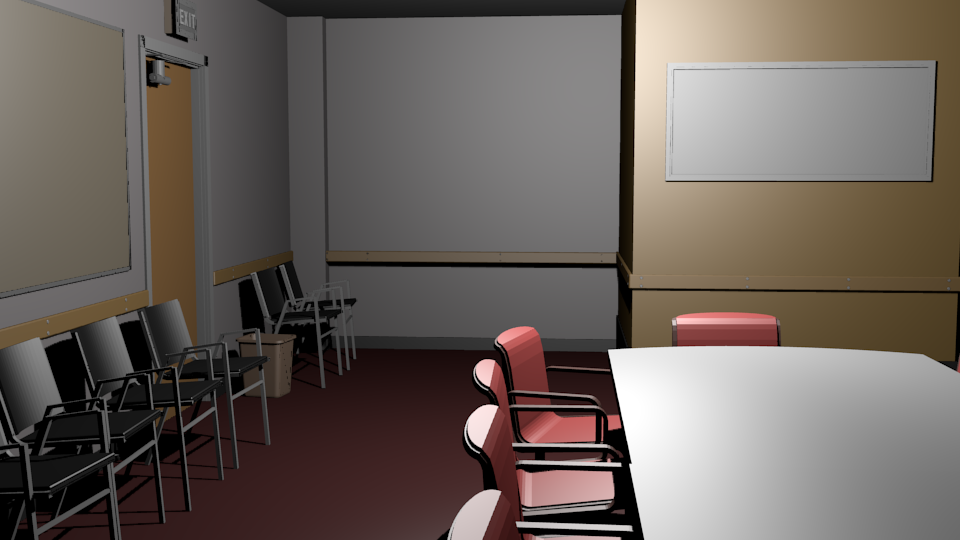
\includegraphics[width=11.5cm,keepaspectratio]{pics/shadows/whyShadows/conferenceShadows}
  \end{figure}
\end{frame}

\begin{frame}\frametitle{Types of light sources / Druhy světel}
  \begin{itemize}
    \item Omnidirectional point light source.
    \item Spot light source.
    \item Directional light source.
  \end{itemize}
  \begin{figure}[h]
    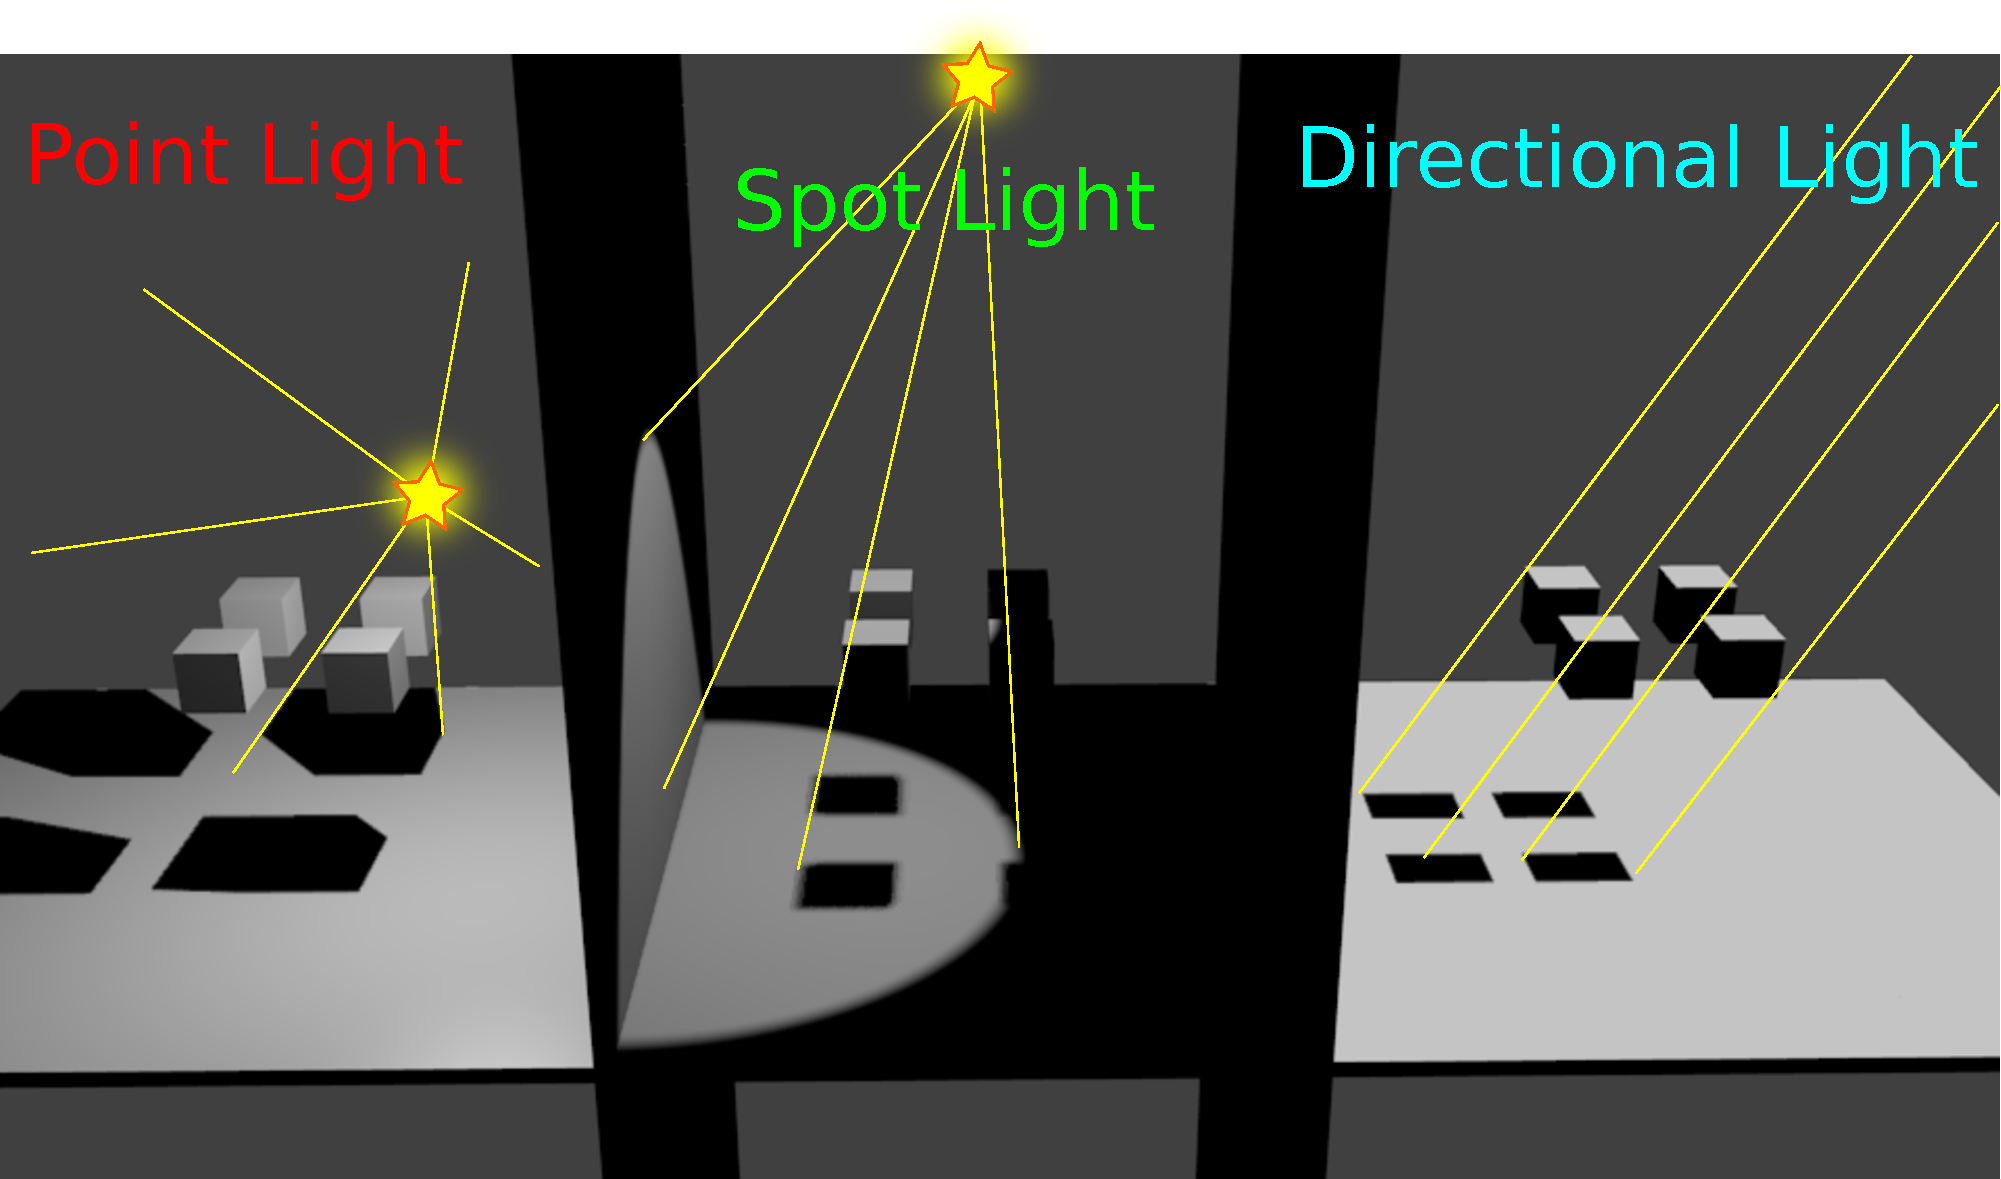
\includegraphics[width=10.5cm,keepaspectratio]{pics/shadows/lightTypes/lightTypes.pdf}
  \end{figure}
\end{frame}

\begin{frame}\frametitle{Types of shadows / Druhy stínů}\scriptsize
  \begin{itemize}
    \item Hard shadows are created by infinitesimal light sources (common in computer graphics).
    \item Soft shadow are created from area light sources.
  \end{itemize}
  \begin{itemize}
    \item Tvrdé stíný vznikají z nekonečně malých světelných zdrojů (časté v počítačové grafice).
    \item Měkké stíny vznikají z plošných zdrojů světla.
  \end{itemize}
  \begin{figure}[h]
    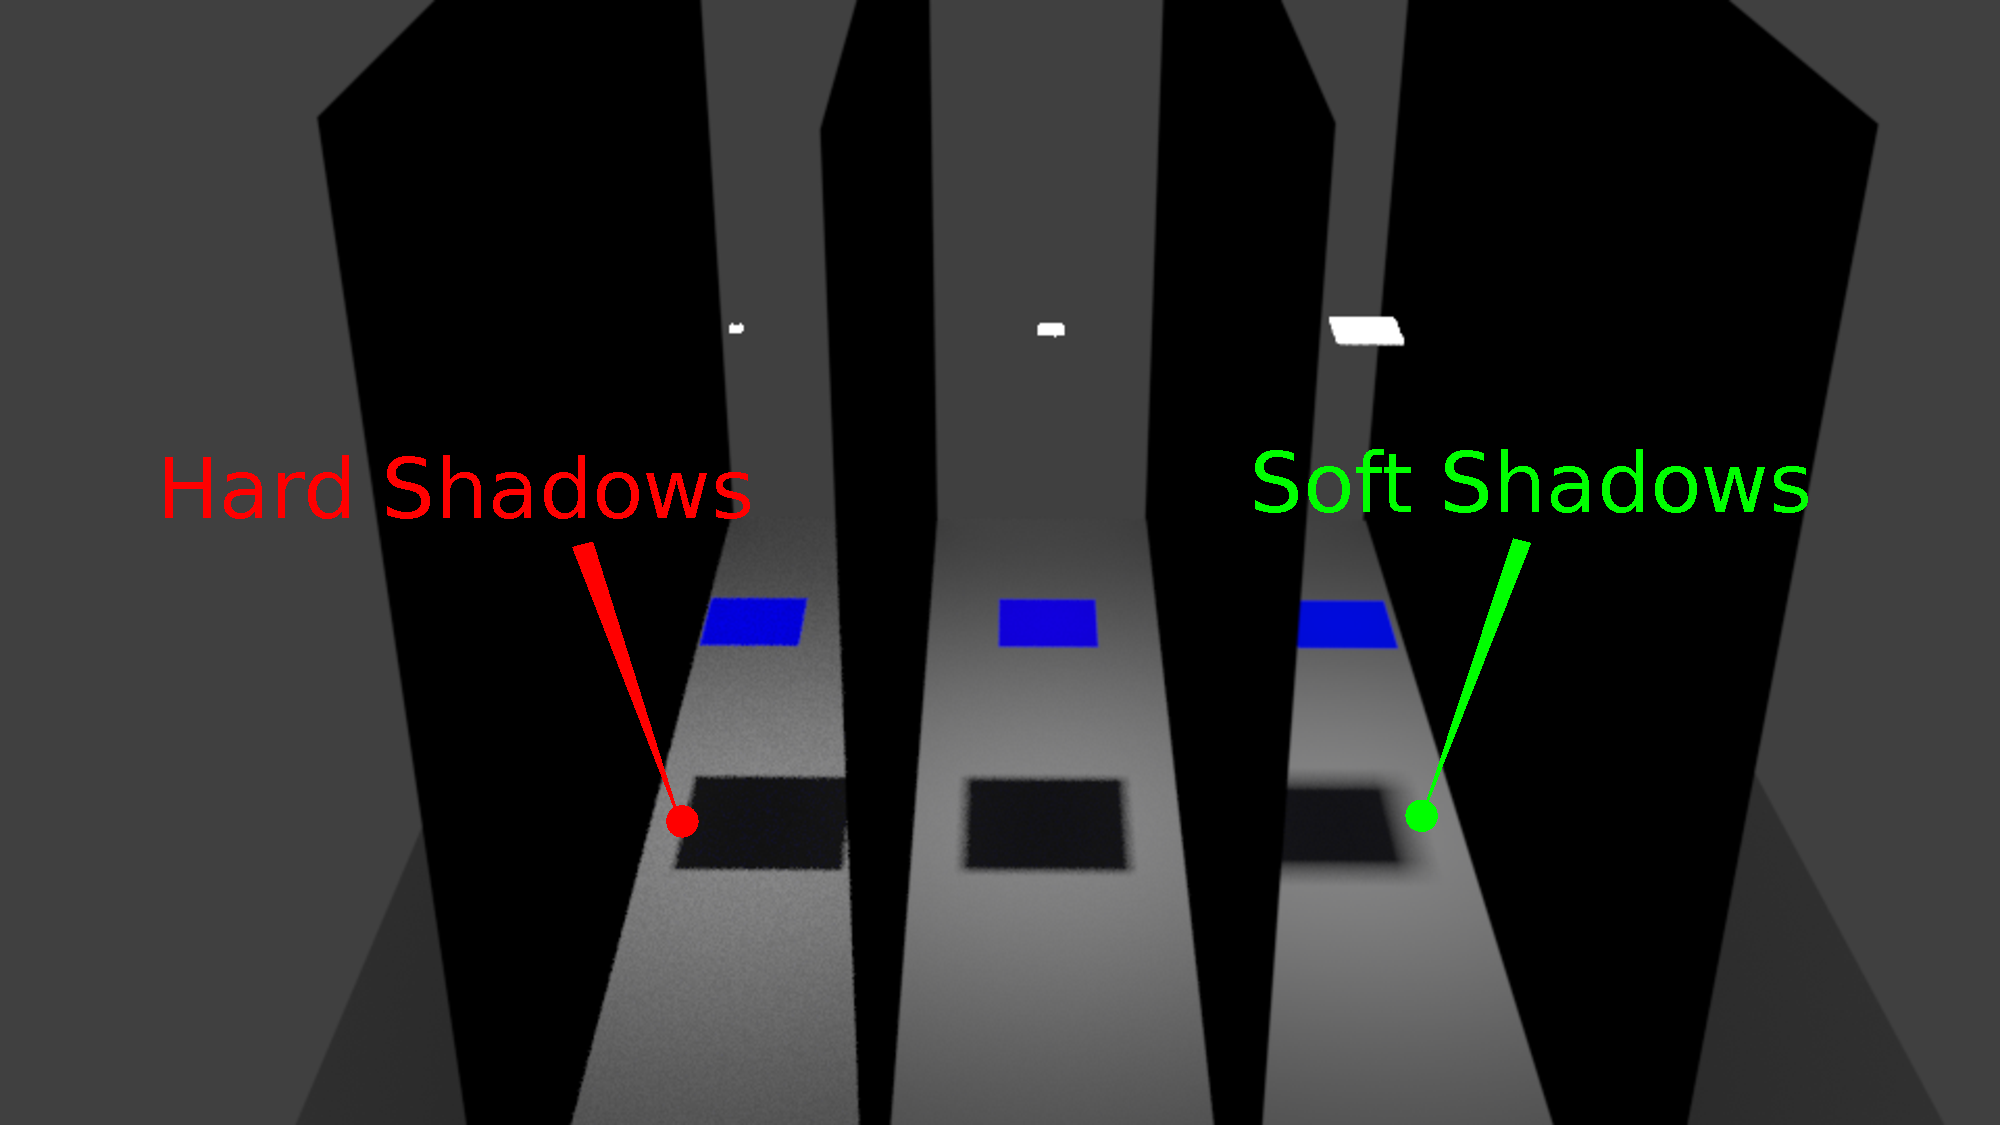
\includegraphics[width=11cm,keepaspectratio]{pics/shadows/hardShadow/hardShadow.pdf}
  \end{figure}
\end{frame}

\begin{frame}\frametitle{Types of shadows / Druhy stínů}\scriptsize
  \begin{itemize}
    \item Fully lit parts of the scene see all points of the light source.
    \item Fully shadowed parts of the scene do not see any point of the light source.
    \item Half shadow (penumbra) is created in regions with partial visibility to the light source.
  \end{itemize}
  \begin{figure}[h]
    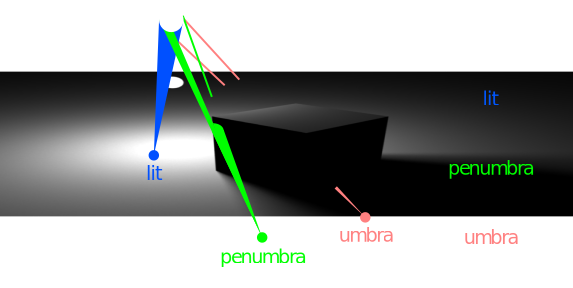
\includegraphics[width=11cm,keepaspectratio]{pics/shadows/penumbra/penumbra}
  \end{figure}
\end{frame}

\begin{frame}\frametitle{Types of shadows / Druhy stínů}\scriptsize
  \begin{itemize}
    \item Shadows are created from direct illumination (can be hard, if the light source is small).
    \item Shadows are created from indirect illumination (soft shadows).
  \end{itemize}
  \begin{itemize}
    \item Stíny vznikají z přímého osvětlení (můžou být tvrdé, pokud je světlo malé).
    \item Stíny vznikají z nepřímého osvětlení (měkké stíny).
  \end{itemize}
  \begin{figure}[h]
    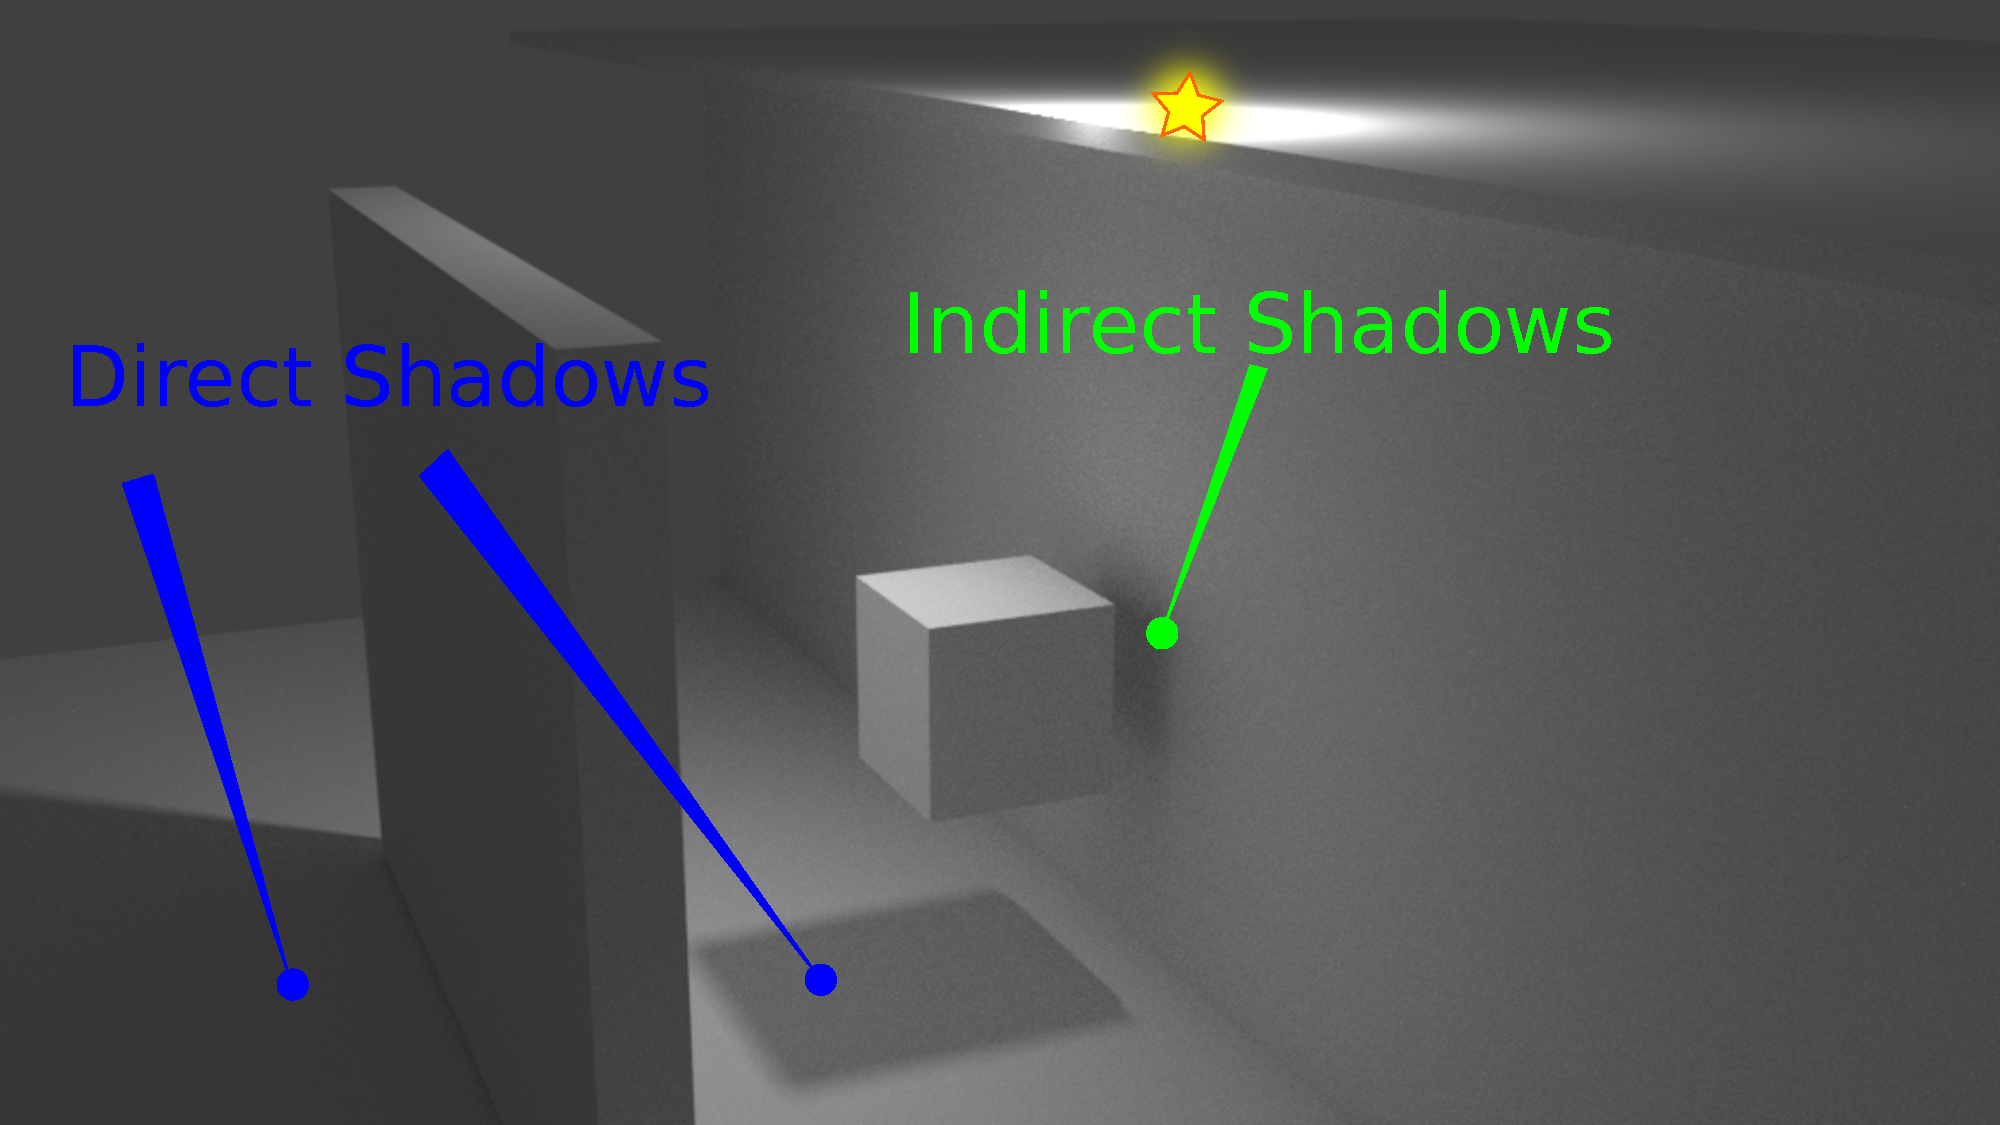
\includegraphics[width=11cm,keepaspectratio]{pics/shadows/indirectShadow/indirectShadows.pdf}
  \end{figure}
\end{frame}

\begin{frame}\frametitle{Ambient occlusion}
  \begin{itemize}
    \item Ambient occlusion - approximation of global illumination.
    \item Ambient occlusion - metoda pro aproximaci části globálního osvětlení a simulaci stínů nepřímého osvětlení.
  \end{itemize}
  \begin{figure}[h]
    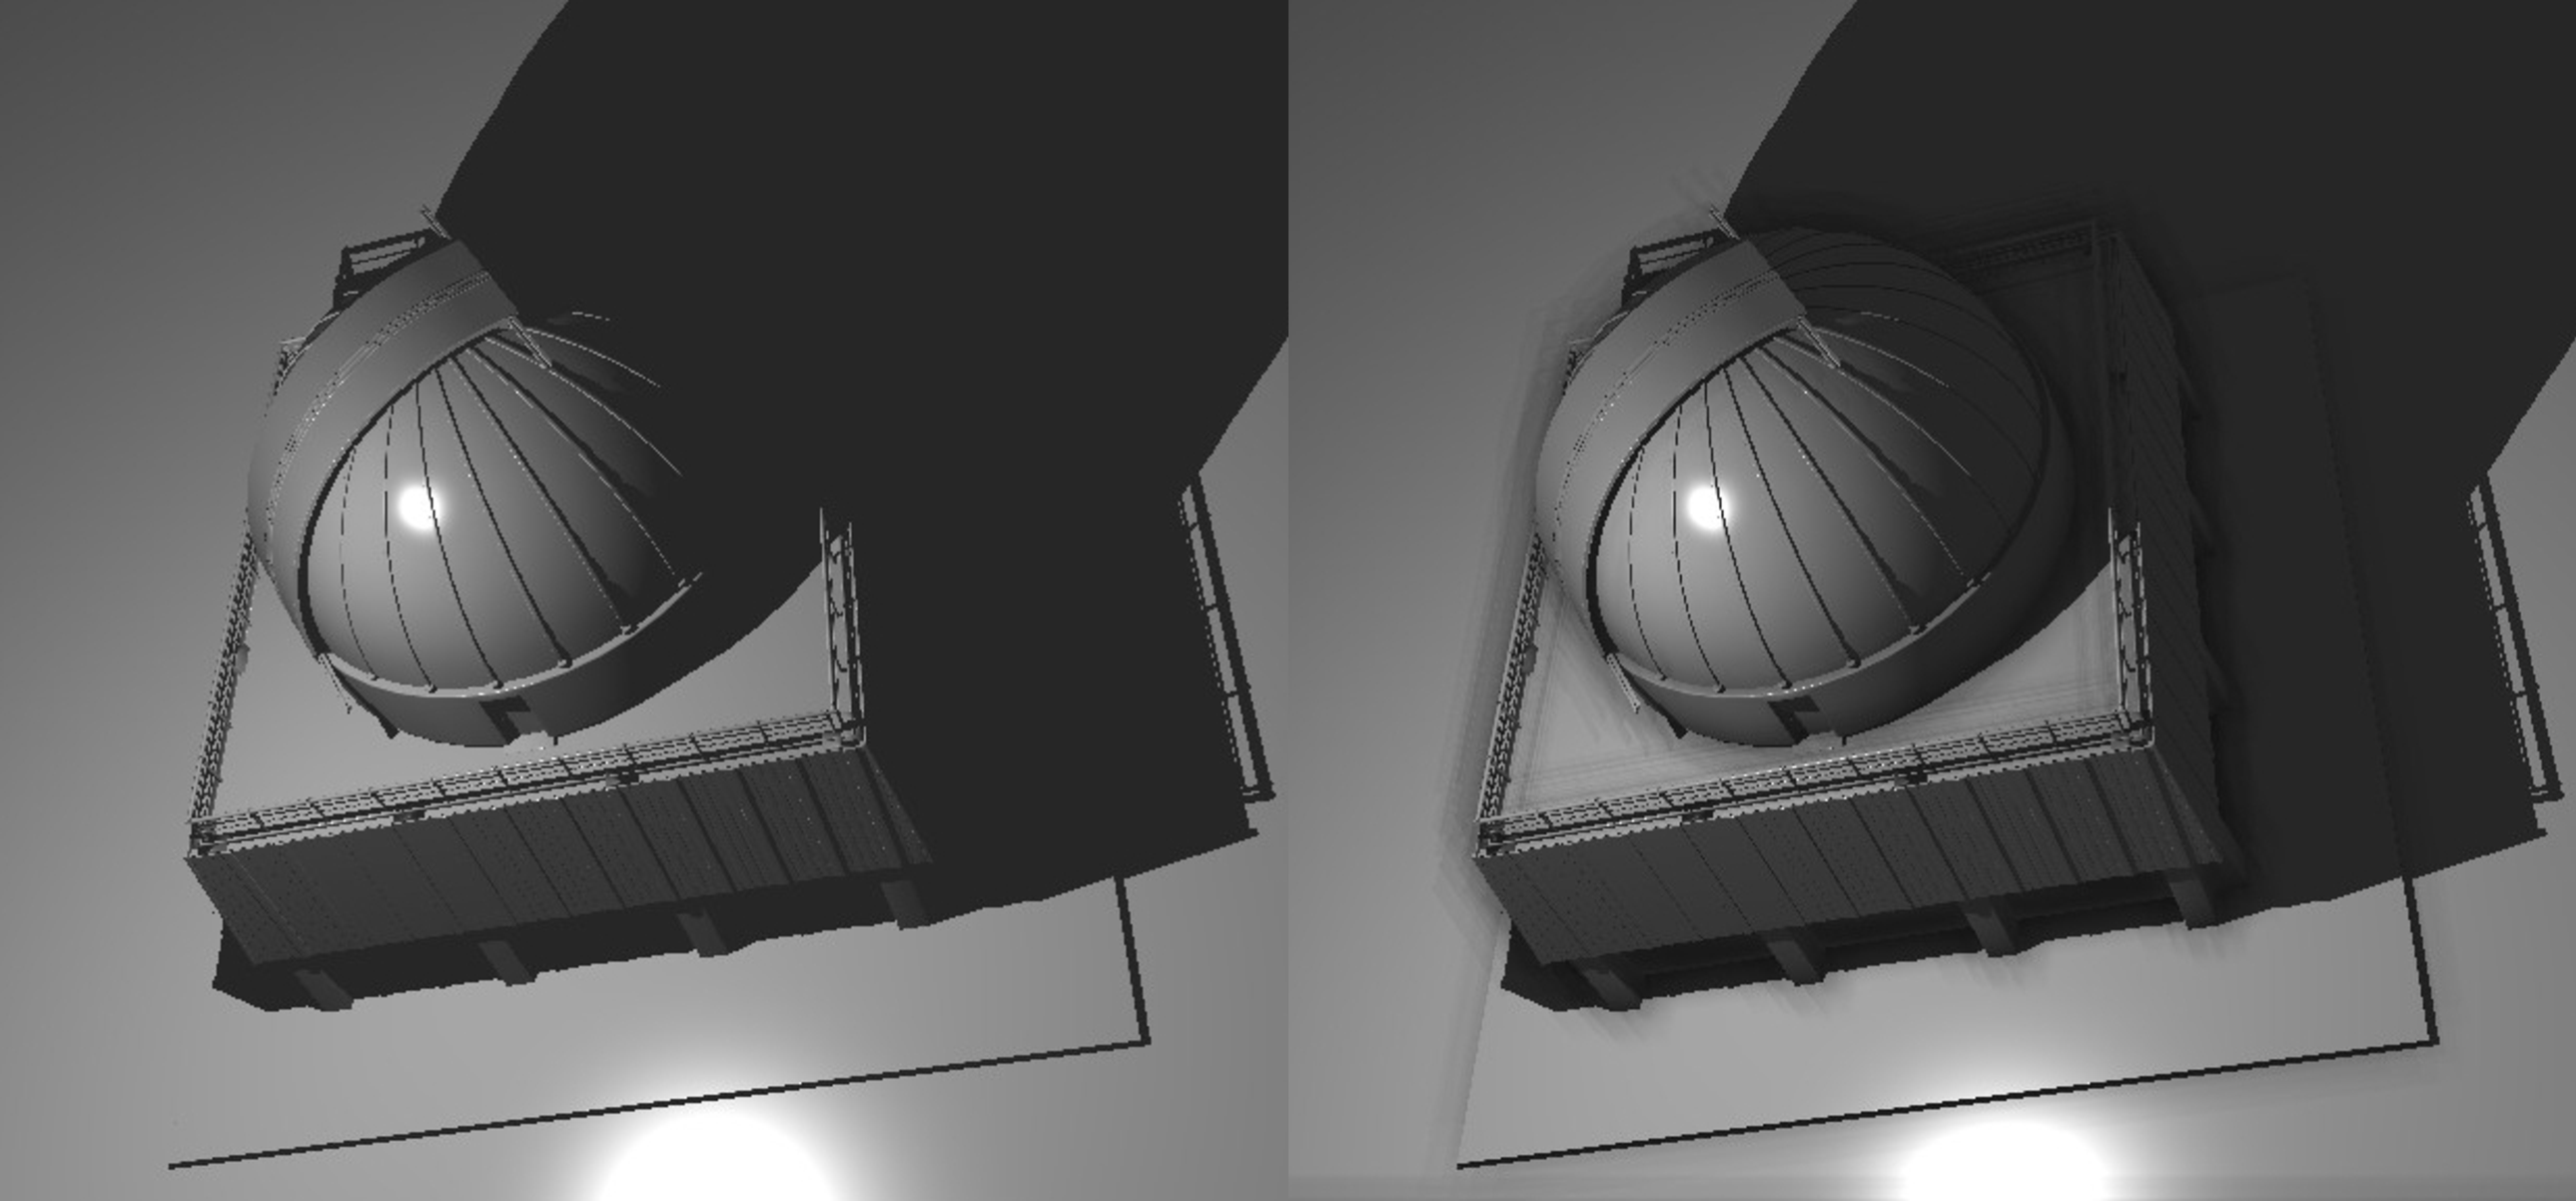
\includegraphics[width=11.5cm,keepaspectratio]{pics/shadows/ambientOcclusion/difference}
  \end{figure}
\end{frame}

\begin{frame}\frametitle{Ambient occlusion}
  \begin{figure}[h]
    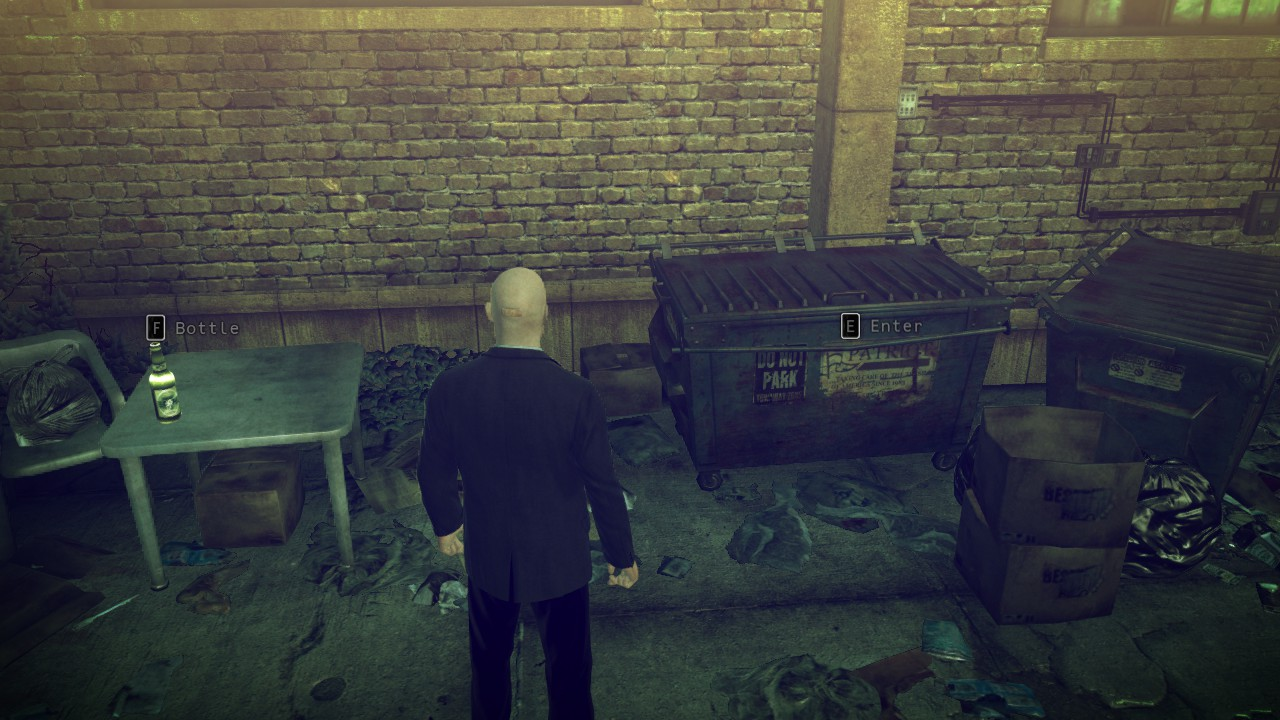
\includegraphics[width=11.5cm,keepaspectratio]{pics/shadows/ambientOcclusion/hitman}
  \end{figure}
\end{frame}

\begin{frame}\frametitle{Ambient occlusion}
  \begin{figure}[h]
    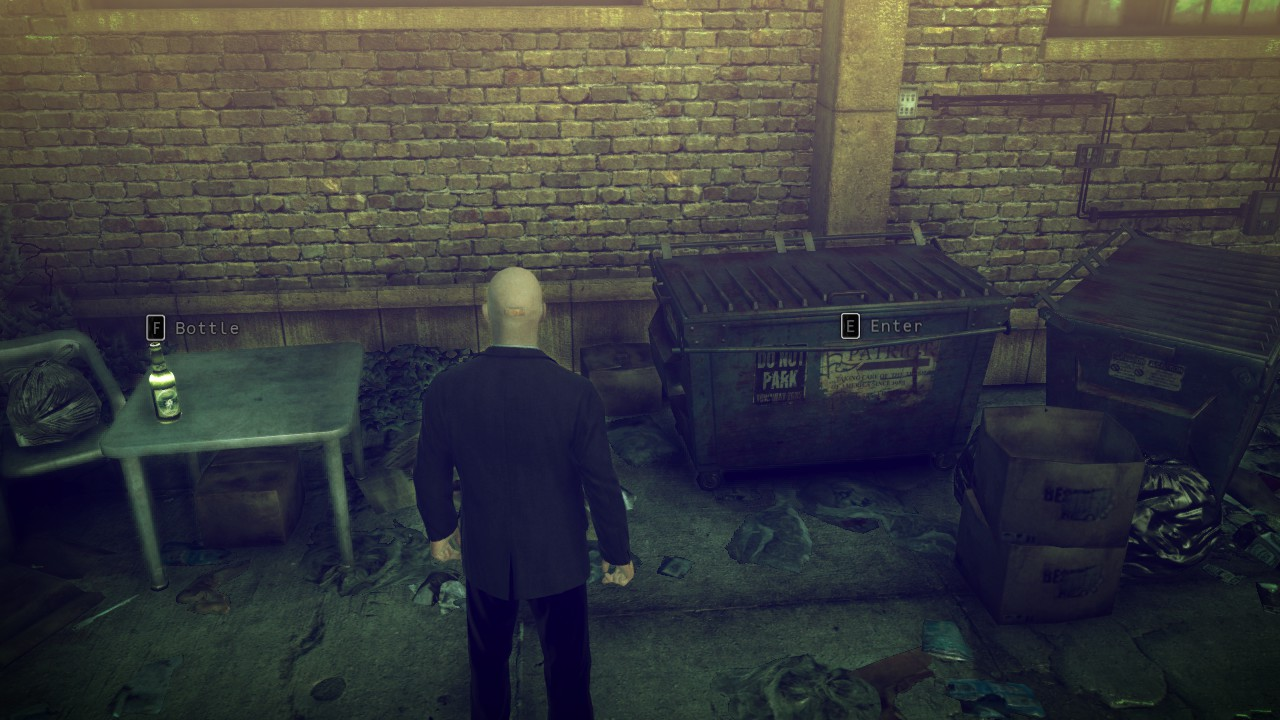
\includegraphics[width=11.5cm,keepaspectratio]{pics/shadows/ambientOcclusion/hitmanssao}
  \end{figure}
\end{frame}

\begin{frame}\frametitle{Ambient occlusion}
  \begin{figure}[h]
    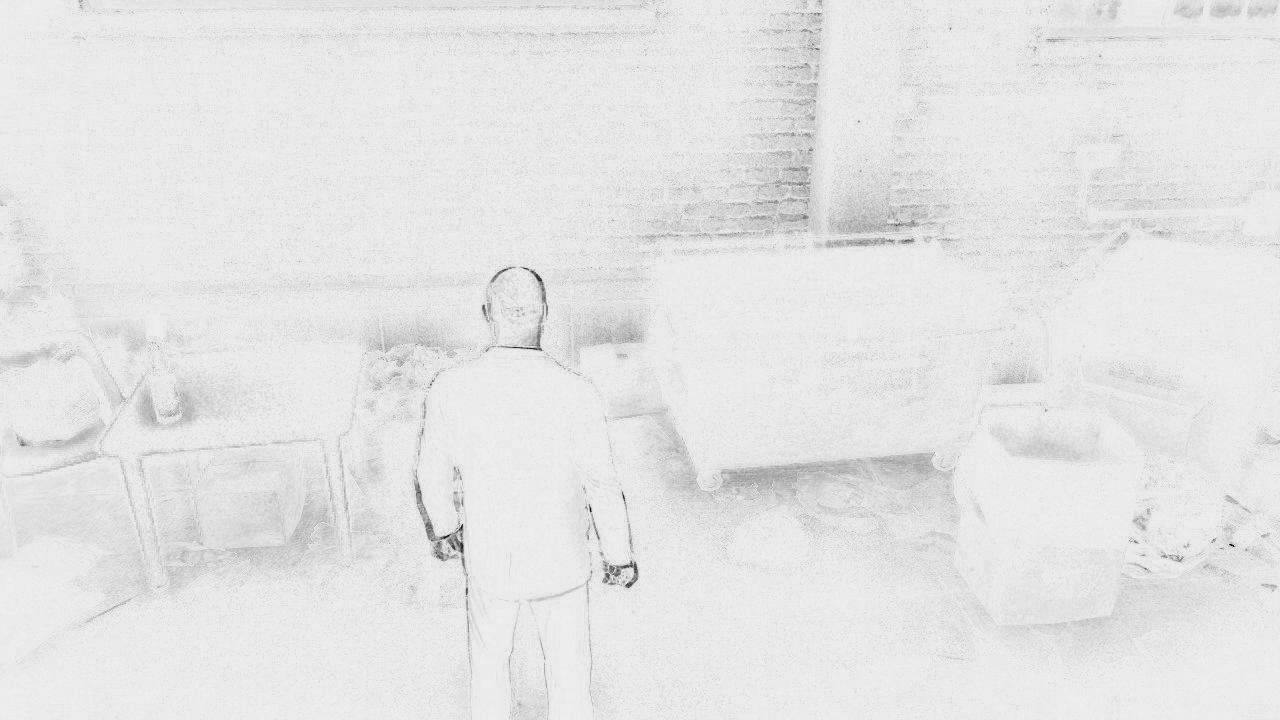
\includegraphics[width=11.5cm,keepaspectratio]{pics/shadows/ambientOcclusion/hitmanDifference}
  \end{figure}
\end{frame}

\setbeamercolor{background canvas}{bg=fitblue}
\begin{frame}
  \frametitle{Shadow volumes}
  \begin{center}
    \Huge {\color{white}Shadow volumes}
  \end{center}
\end{frame}
\setbeamercolor{background canvas}{bg=white}

\begin{frame}[fragile]
  \frametitle{Stencil buffer}

  \begin{itemize}
    \item Další část framebuferu
    \item Celočíselný, obvykle 8bpp
  \end{itemize}
  \vfill

  \begin{minted}[frame=lines]{c++}
    SDL_GL_StencilSize(8);
    glClear(GL_STENCIL_BUFFER_BIT);
    glClearStencil(0);
    glStencilMaskSeparate(GL_FRONT_AND_BACK,~0); //!!!
  \end{minted}
\end{frame}

\begin{frame}[fragile]
  \frametitle{Stencil test}

  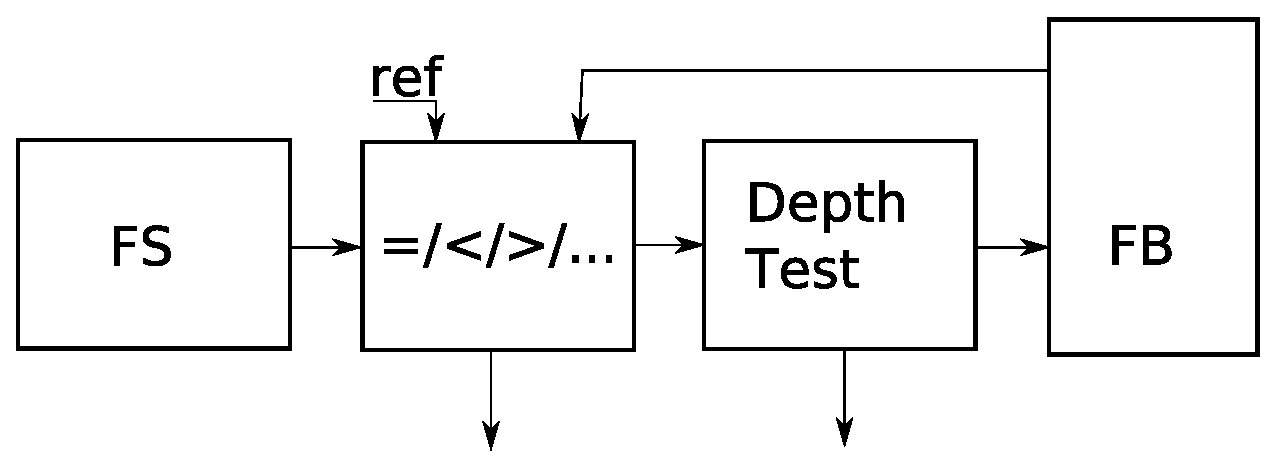
\includegraphics[width=\textwidth]{pics/shadows/shadowVolumes/stencil-test.eps}

  \vfill

  \begin{minted}[frame=lines]{c++}
    glEnable(GL_STENCIL_TEST);

    glStencilFuncSeparate(face, func, ref, mask);
  \end{minted}

  \vfill
  \begin{itemize}
    \item func $\in$ \{GL\_ALWAYS, GL\_NEVER, GL\_LESS, GL\_GREATER, ...\}
    \item if(S\&mask == ref\&mask)//GL\_EQUAL
  \end{itemize}
\end{frame}

\begin{frame}
  \frametitle{Změny stencil bufferu}

  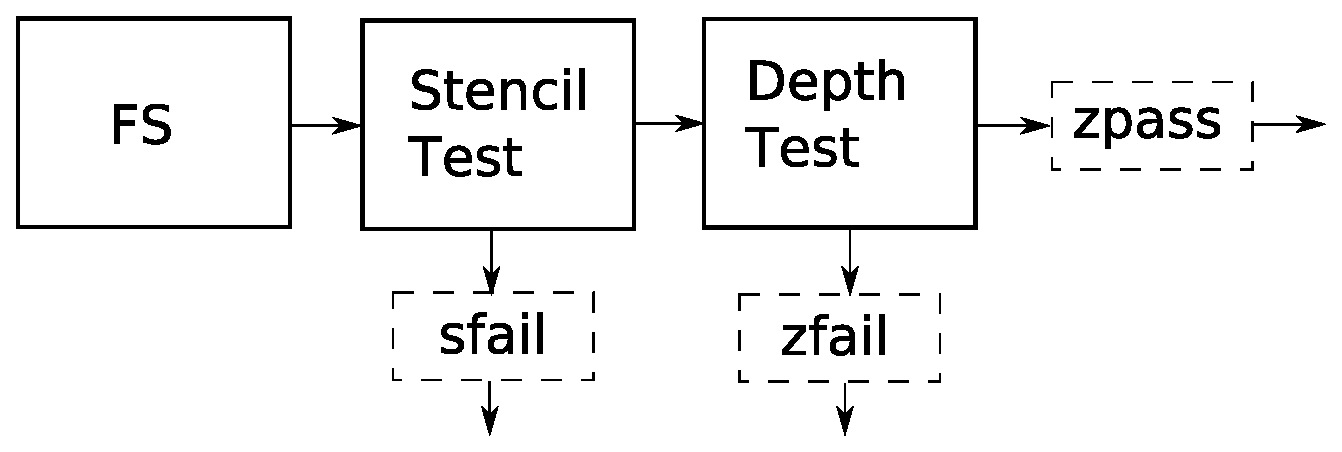
\includegraphics[width=\textwidth]{pics/shadows/shadowVolumes/stencil-test2.eps}

  \vfill

  glStencilOpSeparate(face, sfail, zfail, zpass);

  \begin{itemize}
    \item GL\_KEEP, GL\_ZERO, GL\_REPLACE, GL\_INVERT
    \item GL\_INCR, GL\_DECR, GL\_INCR\_WRAP, GL\_DECR\_WRAP
  \end{itemize}

  \vfill

  $255 + 1 = 255 \Longleftrightarrow $ GL\_INCR

  $255 + 1 = 0 \Longleftrightarrow $ GL\_INCR\_WRAP

\end{frame}




\begin{frame}
  \frametitle{Shadow Volumes}
  \begin{itemize}
    \item Shadow volume je metoda pro tvorbu přesných tvrdých stínů.
    \item Vyžaduje 3 kreslící průchody.
    \item První průchod - vykreslení scény pouze s ambientním světlem.
    \item Druhý průchod - vykreslení stínové geometrie a vytvoření stencilové masky.
    \item Třetí průchod - vykreslení scény s difuzním a spekulárním světlem s využitím stencilové masky.
    \item Existují dvě verze: zpass a zfail.
  \end{itemize}
\end{frame}

\begin{frame}
  \frametitle{Shadow Volumes algoritmus}
  \begin{enumerate}
    \item 1. kreslící průchod - ambietní světlo
      \begin{enumerate}
        \item Vykresli scénu s ambietním osvětlením.
      \end{enumerate}
    \item 2. kreslící průchod - tvorba stencilové masky
      \begin{enumerate}
        \item Vypni kreslení barvy a modifikaci depth bufferu.
        \item Nastav stencilovou operaci na incrementaci u přivrácených trojúhelníku a dekrementaci při odvrácených trojúhelníků.
        \item Povol zápis do stencil bufferu.
        \item Vykresli stínovou geometrii - vytvoří se stencilová maska.
        \item Vypni zápis do stencilového bufferu.
        \item Povol kreslení barvy a modifikaci depth bufferu.
      \end{enumerate}

    \item 3. kreslící průchod - difuzní, spekulární svetlo
      \begin{enumerate}
        \item Zapni stencil test -  při stencilové hodnotě 0 test projde.
        \item Vykresli scénu s difuzním a spekuláním osvětlením.
        \item Vypni stencil test.
      \end{enumerate}
  \end{enumerate}
\end{frame}

\begin{frame}
    \frametitle{Jak na stínová tělesa?}

    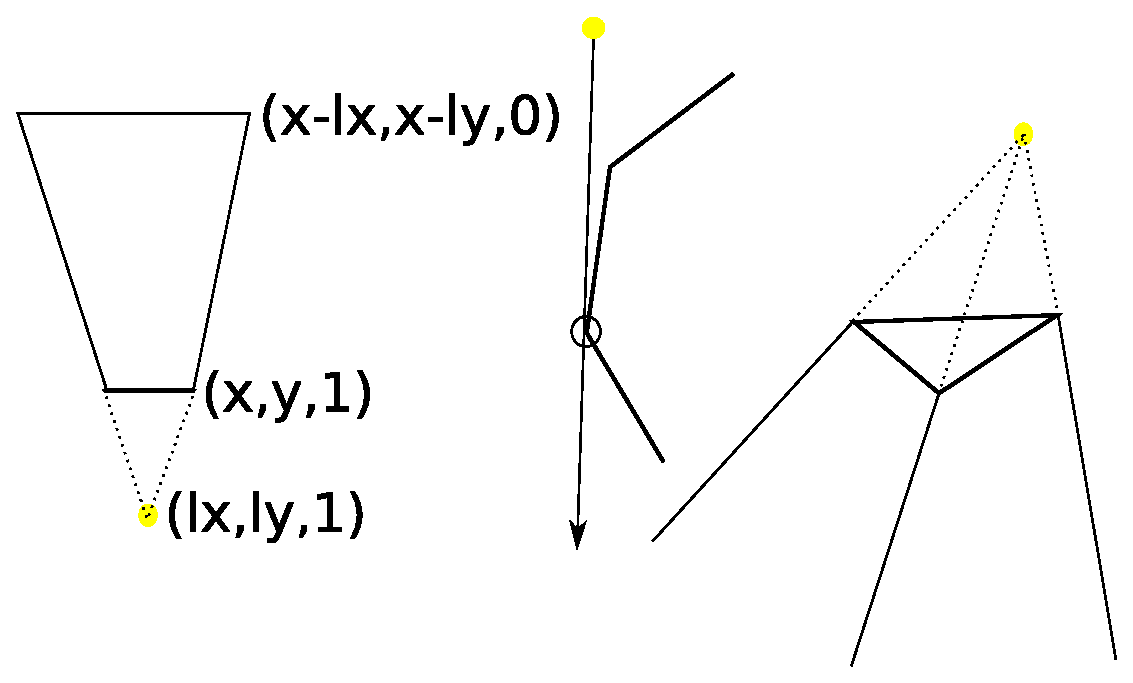
\includegraphics[width=\textwidth]{pics/shadows/shadowVolumes/shom.eps}

    \vfill

    \begin{itemize}
        \item Siluetu protáhnout do nekonečna
        \item Ideální bod $(x,y,z,0)$
    \end{itemize}
\end{frame}

\begin{frame}[fragile]
  \frametitle{Shadow volumes - tvorba geometrie}
  \begin{columns}[T]
    \begin{column}{.44\textwidth}
      {\tiny
        \begin{minted}[frame=lines]{glsl}
          #version 330
          layout(triangles)in;
          layout(triangle_strip,max_vertices=10)out;
          uniform mat4 MVP,M;//matice
          uniform vec4 LightPosition;//pozice svetla
          void main(){
            vec4 LP=M*LightPosition;
            vec4 p[6];
            p[0]=gl_in[0].gl_Position;//body trojuhelniku
            p[1]=gl_in[1].gl_Position;
            p[2]=gl_in[2].gl_Position;
            p[3]=vec4(gl_in[0].gl_Position.xyz*LP.w-LP.xyz,0);//v nekonecnu
            p[4]=vec4(gl_in[1].gl_Position.xyz*LP.w-LP.xyz,0);
            p[5]=vec4(gl_in[2].gl_Position.xyz*LP.w-LP.xyz,0);
            vec3 N=normalize(cross((p[1]-p[0]).xyz,(p[2]-p[0]).xyz));
            float Distance=dot(N,LP.xyz)-dot(N,p[0].xyz);
            if(Distance<=0){//otocime volume vnitrkem ven
              vec4 c=p[0];p[0]=p[1];p[1]=c;
              c=p[3];p[3]=p[4];p[4]=c;
            }
            gl_Position=MVP*p[0];EmitVertex();
            gl_Position=MVP*p[1];EmitVertex();
            gl_Position=MVP*p[3];EmitVertex();
            gl_Position=MVP*p[4];EmitVertex();
            gl_Position=MVP*p[5];EmitVertex();
            gl_Position=MVP*p[1];EmitVertex();
            gl_Position=MVP*p[2];EmitVertex();
            gl_Position=MVP*p[0];EmitVertex();
            gl_Position=MVP*p[5];EmitVertex();
            gl_Position=MVP*p[3];EmitVertex();
            EndPrimitive();
          }
        \end{minted}
      }
    \end{column}
    \begin{column}{.48\textwidth}
      \begin{figure}[h]
        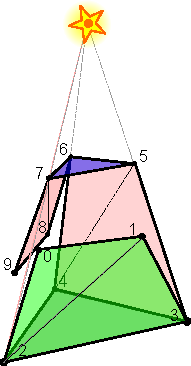
\includegraphics[width=3cm,keepaspectratio]{pics/shadows/shadowVolumes/perTriangle.pdf}
      \end{figure}
    \end{column}
  \end{columns}

\end{frame}

\begin{frame}
  \frametitle{Shadow Volumes ZPass}
  \begin{figure}[h]
    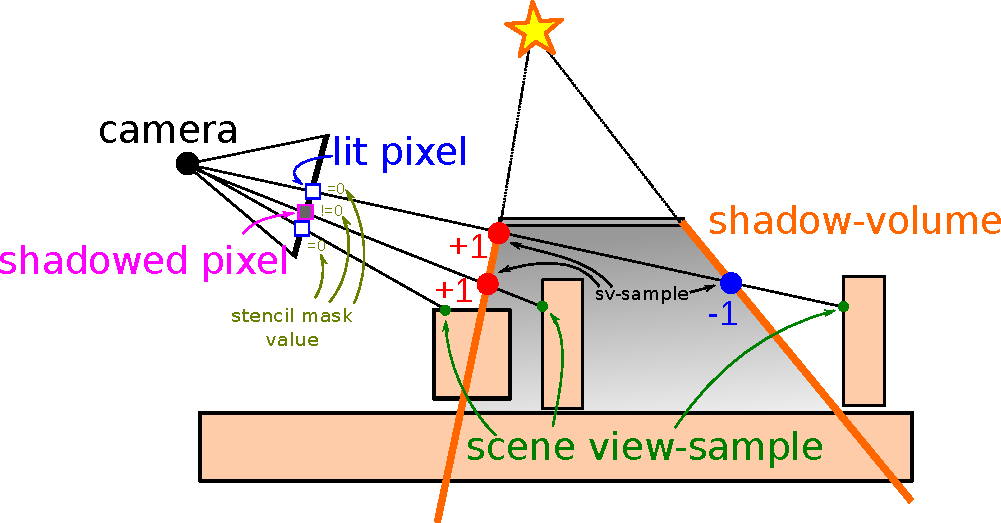
\includegraphics[width=11.5cm,keepaspectratio]{pics/shadows/shadowVolumes/ZPass}
  \end{figure}
\end{frame}

\begin{frame}[fragile]
  \frametitle{Shadow Volumes - 1. průchod}

  \begin{minted}[frame=lines]{c++}
//activate phong program
glUseProgram(phongProgram);

//enable ambient lighting
glProgramUniform4fv(phongProgram,
  lightAmbientColorUniform,light.amientColor);

//disable diffuse and specular lighting
glProgramUniform4f (phongProgram,
  lightDiffuseColorUniform,0,0,0,0);
glProgramUniform4f (phongProgram,
  lightSpecularColorUniform,0,0,0,0);

//draw the scene
glMultiDrawElementsIndirect(...);
  \end{minted}
\end{frame}

\begin{frame}[fragile]
  \frametitle{Shadow Volumes - 2. průchod}

  \begin{minted}[frame=lines]{c++}
//activate shadow volume geometry program
glUseProgram(shadowVolumeProgram);

glColorMask(GL_FALSE,GL_FALSE,GL_FALSE,GL_FALSE);
glDepthMask(GL_FALSE);

glEnable(GL_STENCIL_TEST);
glStencilFunc(GL_ALWAYS,0,0);
glStencilOpSeparate(GL_FRONT,GL_KEEP,GL_KEEP,GL_INCR_WRAP);
glStencilOpSeparate(GL_BACK ,GL_KEEP,GL_KEEP,GL_DECR_WRAP);

//draw the shadow geometry
glMultiDrawElementsIndirect(...);

glStencilOp(GL_KEEP,GL_KEEP,GL_KEEP);
glDepthMask(GL_TRUE);
glColorMask(GL_TRUE,GL_TRUE,GL_TRUE,GL_TRUE);
  \end{minted}
\end{frame}

\begin{frame}[fragile]
  \frametitle{Shadow Volumes - 3. průchod}

  \begin{minted}[frame=lines]{c++}
//activate phong program
glUseProgram(shadowVolumeProgram);

glProgramUniform4f (phongProgram,
  lightAmbientColorUniform,0,0,0,0);
glProgramUniform4f (phongProgram,
  lightDiffuseColorUniform,light.diffuseColor);
glProgramUniform4f (phongProgram,
  lightSpecularColorUniform,light.specularColor);

glStencilFunc(GL_EQUAL,0,0xff);

//draw the scene
glMultiDrawElementsIndirect(...);

glDisable(GL_STENCIL_TEST);
  \end{minted}
\end{frame}


\begin{frame}
    \frametitle{Víc světel}
    $N$ světel znamená $2^N$ kombinací zastíněností :( Co s tím?
    \pause\vfill
    \begin{equation*}
        \begin{array}{lcll}
            L &=& k_e + \sum\limits_{i=1}^n k_a \cdot L_{a(i)}   & + k_d \cdot L_{d(i)} \cdot (\vec L_i \cdot \vec N) + k_s \cdot L_{s(i)} \cdot (\vec V \cdot \vec{R_i})^n \\
            L_0 &=& k_e + \sum\limits_{i=1}^n k_a \cdot L_{a(i)} & \\
            L_i &=& L_{i-1}                                      & + k_d \cdot L_{d(i)} \cdot (\vec L_i \cdot \vec N) + k_s \cdot L_{s(i)} \cdot (\vec V \cdot \vec{R_i})^n
        \end{array}
    \end{equation*}
    \pause\vfill
    \begin{itemize}
        \item Vykreslit scénu s ambient+emission
        \item Pro každé světlo
        \begin{itemize}
            \item Připravit stencil buffer
            \item Přiblendovat diffuse+specular
            \item (glDepthFunc(GL\_LEQUAL), glBlendFunc(GL\_ONE, GL\_ONE))
        \end{itemize}
    \end{itemize}
\end{frame}

\begin{frame}
    \frametitle{Výhody a nevýhody}
    
    $+$
    \begin{itemize}
        \item Dynamické scény
        \item Problematické scény
        \item Sedí na pixel přesně
    \end{itemize}

    \vfill
    $-$
    \begin{itemize}
        \item Pomalé
        \item Závislé na fillrate
        \item Konstrukce stínových těles
        \item Jen ostré stíny
    \end{itemize}
\end{frame}

\begin{frame}
    \frametitle{Problém...}
    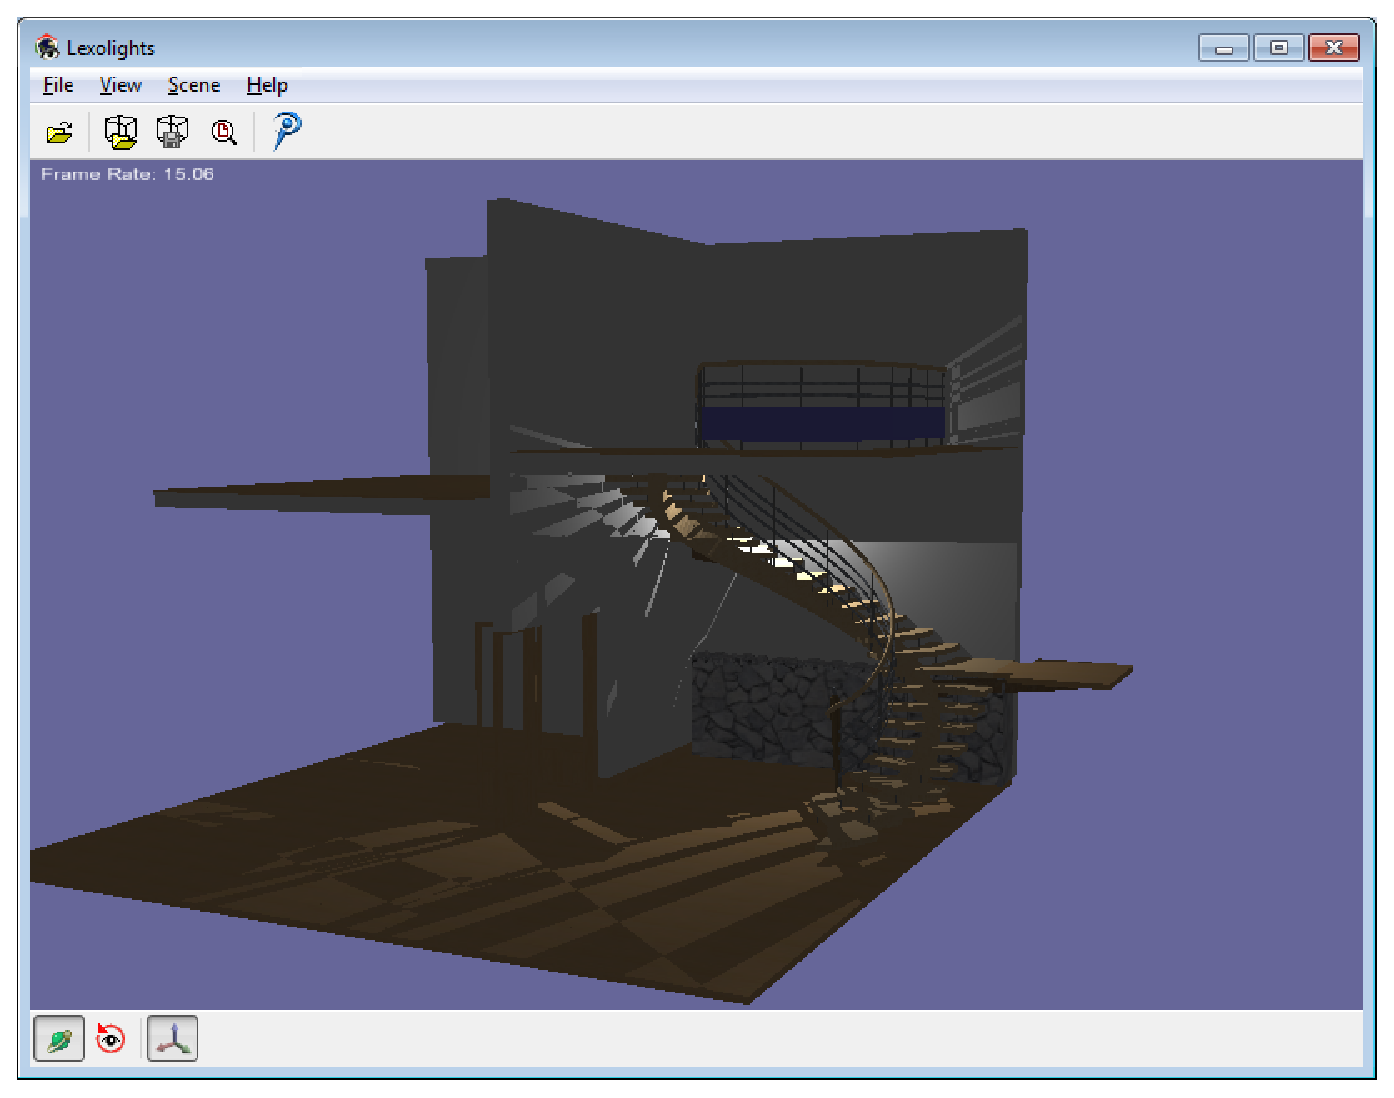
\includegraphics[width=3in]{pics/shadows/shadowVolumes/ZPass-fail.eps}
    \pause\vfill
    Stačí vlézt dovnitř stínového tělesa.
\end{frame}

\begin{frame}
    \frametitle{Z\_PASS vs. Z\_FAIL}
    Pixel je ve stínu když paprsek vletí {\color{red}dovnitř} a nevyletí {\color{blue}ven}.
    \begin{columns}[c]
    \column{.5\textwidth}
        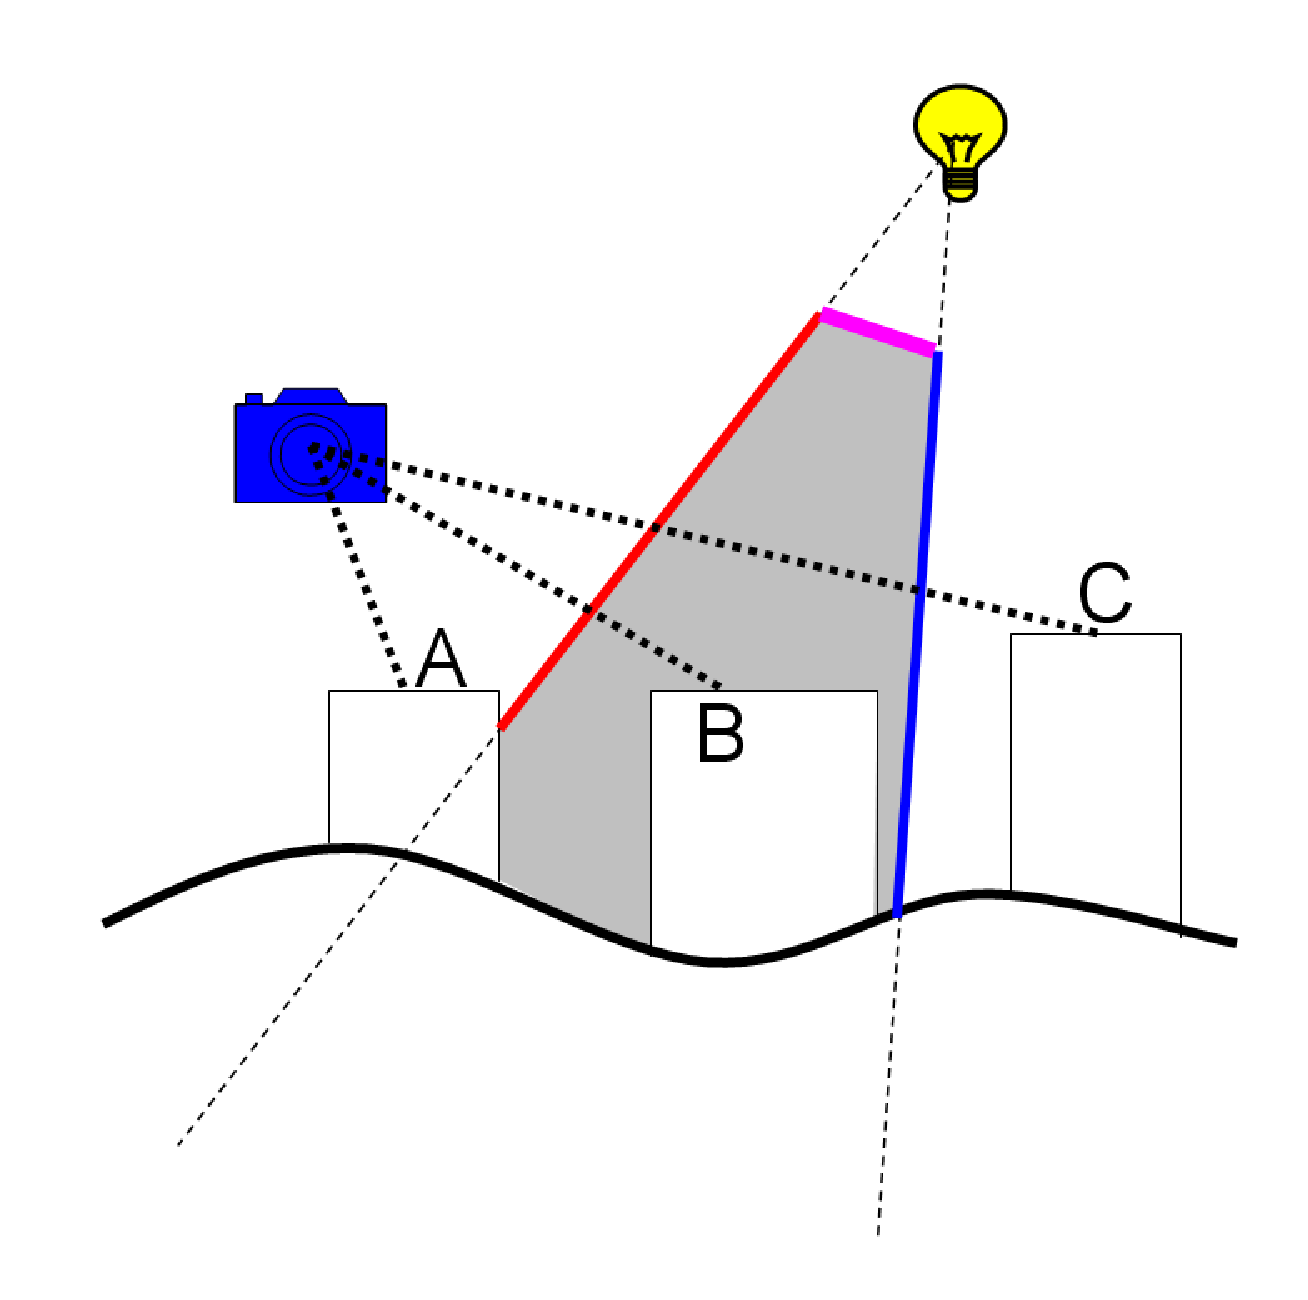
\includegraphics[width=\textwidth]{pics/shadows/shadowVolumes/ShadowVolume.eps}
    \column{.5\textwidth}
        Z\_PASS : \\
        Počítám viditelné pixely \\
        {\color{red} +1}, {\color{blue} -1}
        \vfill
        Z\_FAIL : \\
        Počítám neviditelné pixely
        {\color{red} -1}, {\color{blue} +1}
    \end{columns}
    \pause\vfill
    glStencilOpSeparate(GL\_FRONT, GL\_KEEP, GL\_DECR\_WRAP, GL\_KEEP);\\
    glStencilOpSeparate(GL\_BACK, GL\_KEEP, GL\_INCR\_WRAP, GL\_KEEP);    
\end{frame}

\begin{frame}
    \frametitle{Další zádrhel}
    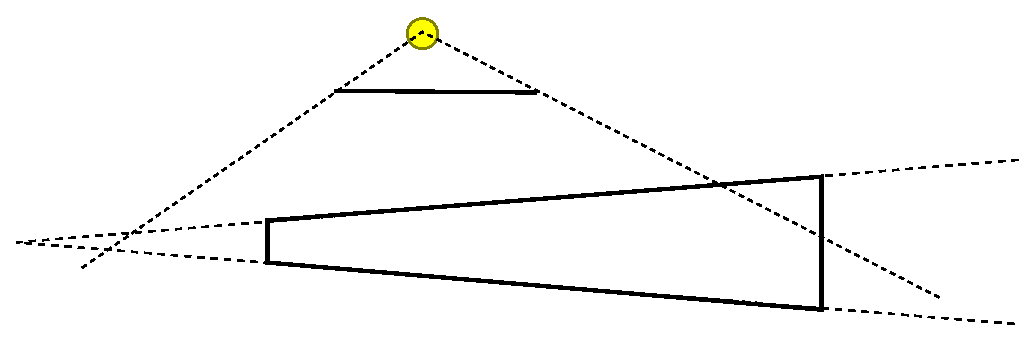
\includegraphics[width=\textwidth]{pics/shadows/shadowVolumes/svol-cap.eps}
    \begin{itemize}
        \item Stínové těleso musí být uzavřené.
        \item A jeho stěny musí být "viditelné".
        \item Problém je far-plane.
    \end{itemize}
\end{frame}

\begin{frame}
  \frametitle{Shadow Volumes ZFail}
  \begin{figure}[h]
    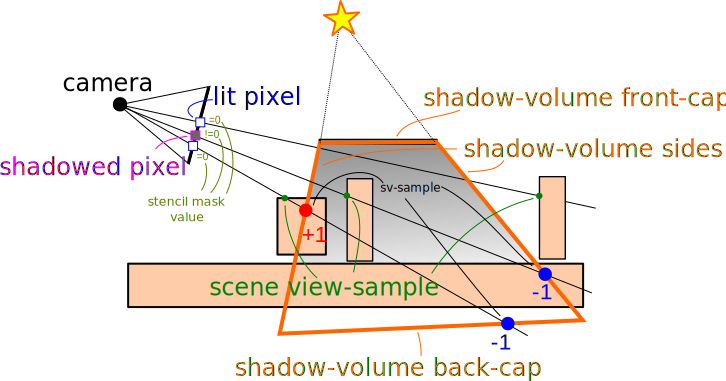
\includegraphics[width=11.5cm,keepaspectratio]{pics/shadows/shadowVolumes/ZFail}
  \end{figure}
\end{frame}

\begin{frame}[fragile]
  \frametitle{Shadow Volumes - 2. průchod modifikace}

  \begin{minted}[frame=lines]{c++}
//activate shadow volume geometry program
glUseProgram(shadowVolumeProgram);
glProgramUniformMatrix4fv(shadowVolumeProgram,mvpUniform,
  1,GL_FALSE,infiniteProjectionMatrix);

glColorMask(GL_FALSE,GL_FALSE,GL_FALSE,GL_FALSE);
glDepthMask(GL_FALSE);

glEnable(GL_STENCIL_TEST);
glStencilFunc(GL_ALWAYS,0,0);
glDepthFunc(GL_LESS);
glStencilOpSeparate(GL_FRONT,GL_KEEP,GL_INCR_WRAP,GL_KEEP);
glStencilOpSeparate(GL_BACK ,GL_KEEP,GL_DECR_WRAP,GL_KEEP);

//draw the shadow geometry with caps
glMultiDrawElementsIndirect(...);

glStencilOp(GL_KEEP,GL_KEEP,GL_KEEP);
glDepthMask(GL_TRUE);
glColorMask(GL_TRUE,GL_TRUE,GL_TRUE,GL_TRUE);
  \end{minted}
\end{frame}


\begin{frame}
    \frametitle{Nekonečná projekce}
    \begin{align*}
        \lim_{\mathrm{far} \to +\infty}\begin{pmatrix}
            \frac{2\mathrm{near}}{\mathrm{right}-\mathrm{left}}&0&\frac{\mathrm{right}+\mathrm{left}}{\mathrm{right}-\mathrm{left}}&0\\
            0&\frac{2\mathrm{near}}{\mathrm{top}-\mathrm{bottom}}&\frac{\mathrm{top}+\mathrm{bottom}}{\mathrm{top}-\mathrm{bottom}}&0\\
            0&0&-\frac{\mathrm{far}+\mathrm{near}}{\mathrm{far}-\mathrm{near}}&-\frac{2\mathrm{near}\mathrm{far}}{\mathrm{far}-\mathrm{near}}\\
            0&0&-1&0
        \end{pmatrix} \\
        = \begin{pmatrix}
            \frac{2\mathrm{near}}{\mathrm{right}-\mathrm{left}}&0&\frac{\mathrm{right}+\mathrm{left}}{\mathrm{right}-\mathrm{left}}&0\\
            0&\frac{2\mathrm{near}}{\mathrm{top}-\mathrm{bottom}}&\frac{\mathrm{top}+\mathrm{bottom}}{\mathrm{top}-\mathrm{bottom}}&0\\
            0&0&-1&-2\mathrm{near}\\
            0&0&-1&0
        \end{pmatrix}
    \end{align*}
    \pause\vfill
    \begin{itemize}
        \item[:)] Vidíme do nekonečna.
        \item[?] Co z-test? Dělíme nekonečnou délku na konečný počet dílků.
    \end{itemize}
\end{frame}

\begin{frame}
    \frametitle{Z-buffer a nekonečno}
    \begin{align*}
        P(z) &= \frac{z - 2n}{z} = 1 - \frac{2n}{z} & \text{ Dopředu je $-z$}
    \end{align*}
    \pause\vfill
    \begin{align*}
        P(n) &= -1 & P(\infty) &=  1 \\
        P(2n) &= 0 & P(4n) &= 1/2
    \end{align*}
    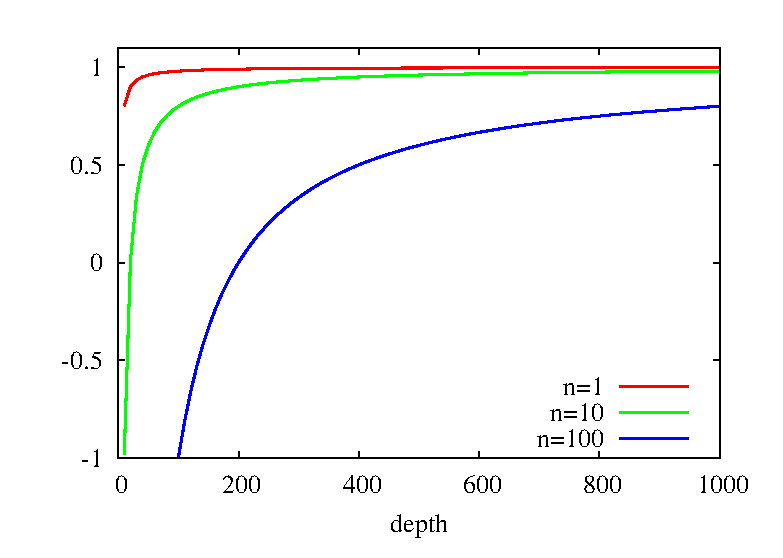
\includegraphics[width=.5\textwidth]{pics/shadows/shadowVolumes/plot/infdepth.eps}
    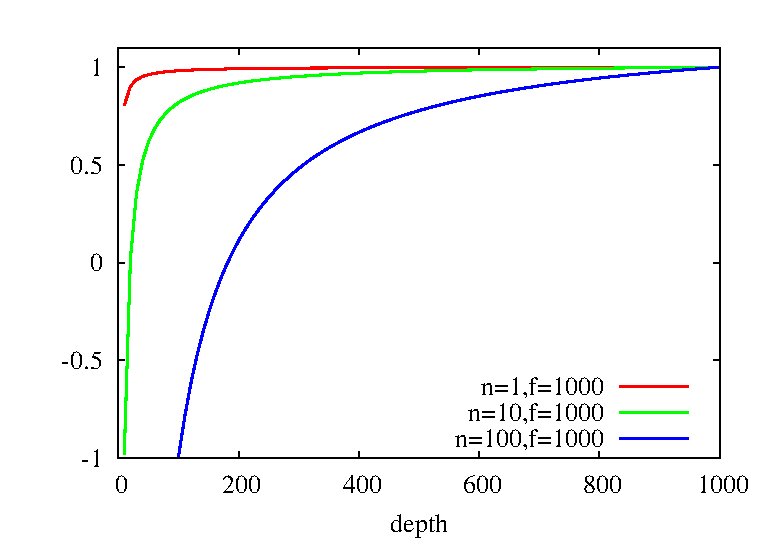
\includegraphics[width=.5\textwidth]{pics/shadows/shadowVolumes/plot/findepth.eps}
    \begin{itemize}
        \item[:)] Většina hodnot z-bufferu je v "rozumné" vzdálenosti.
    \end{itemize}
\end{frame}


\setbeamercolor{background canvas}{bg=fitblue}
\begin{frame}
  \frametitle{Shadow Mapping}
  \begin{center}
    \Huge {\color{white}Shadow Mapping}
  \end{center}
\end{frame}
\setbeamercolor{background canvas}{bg=white}

\begin{frame}
  \frametitle{Shadow-Mapping - přehled}
  \begin{itemize}
    \item Dva průchody
    \item Dva druhy vzorků \\ (view-samples, shadow-samples)
    \item Každý view-sample má přiřazený \\ shadow-sample
  \end{itemize}
  \begin{picture}(320,250)
    \put(135,120){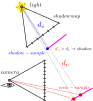
\includegraphics[height=7.5cm,keepaspectratio]{pics/shadows/shadowMapping/shadowmapping}}
    \put(-20,100 ){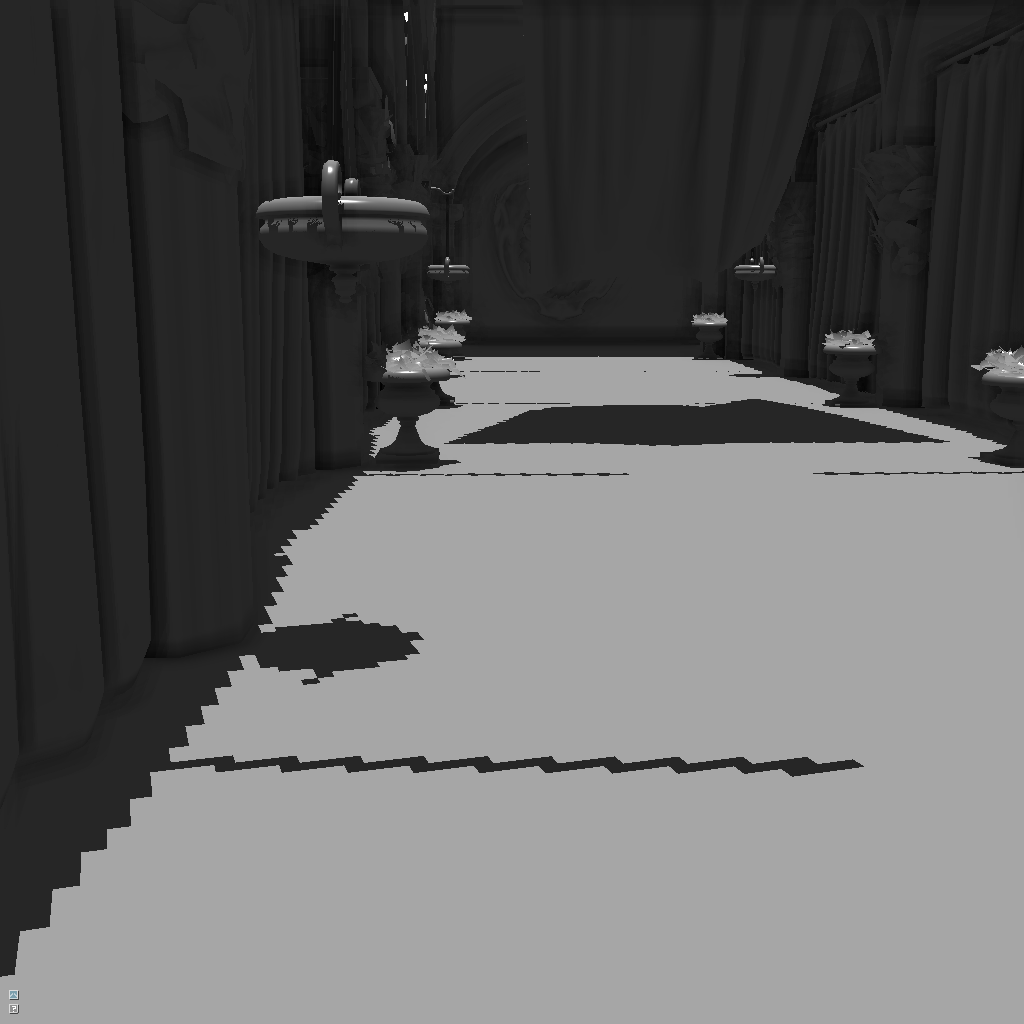
\includegraphics[height=5cm,keepaspectratio]{pics/shadows/shadowMapping/sponza2_sm}}
  \end{picture}
\end{frame}



\begin{frame}
    \frametitle{Stínové mapy}

%    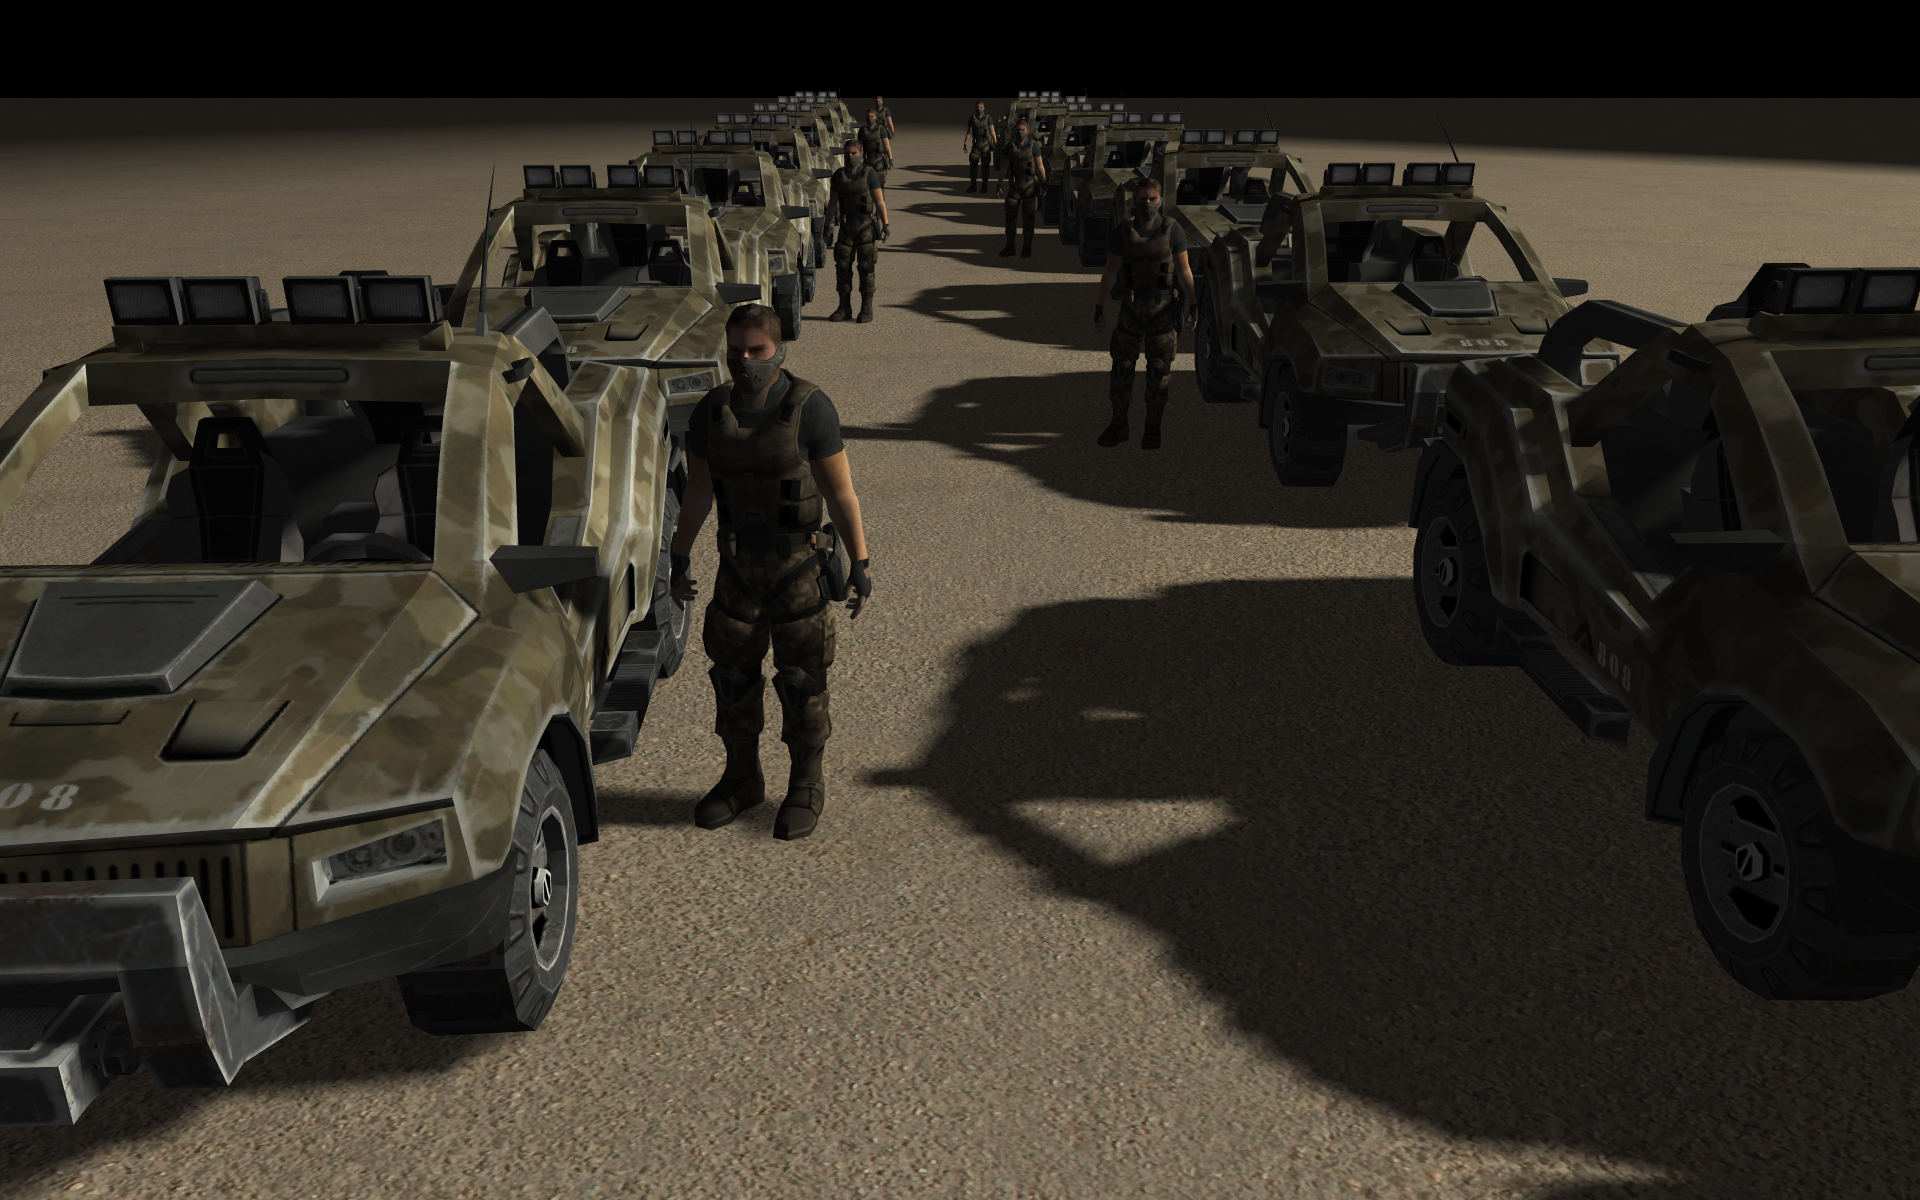
\includegraphics[width=\textwidth]{pics/shadows/shadowMapping/vsm.eps}
    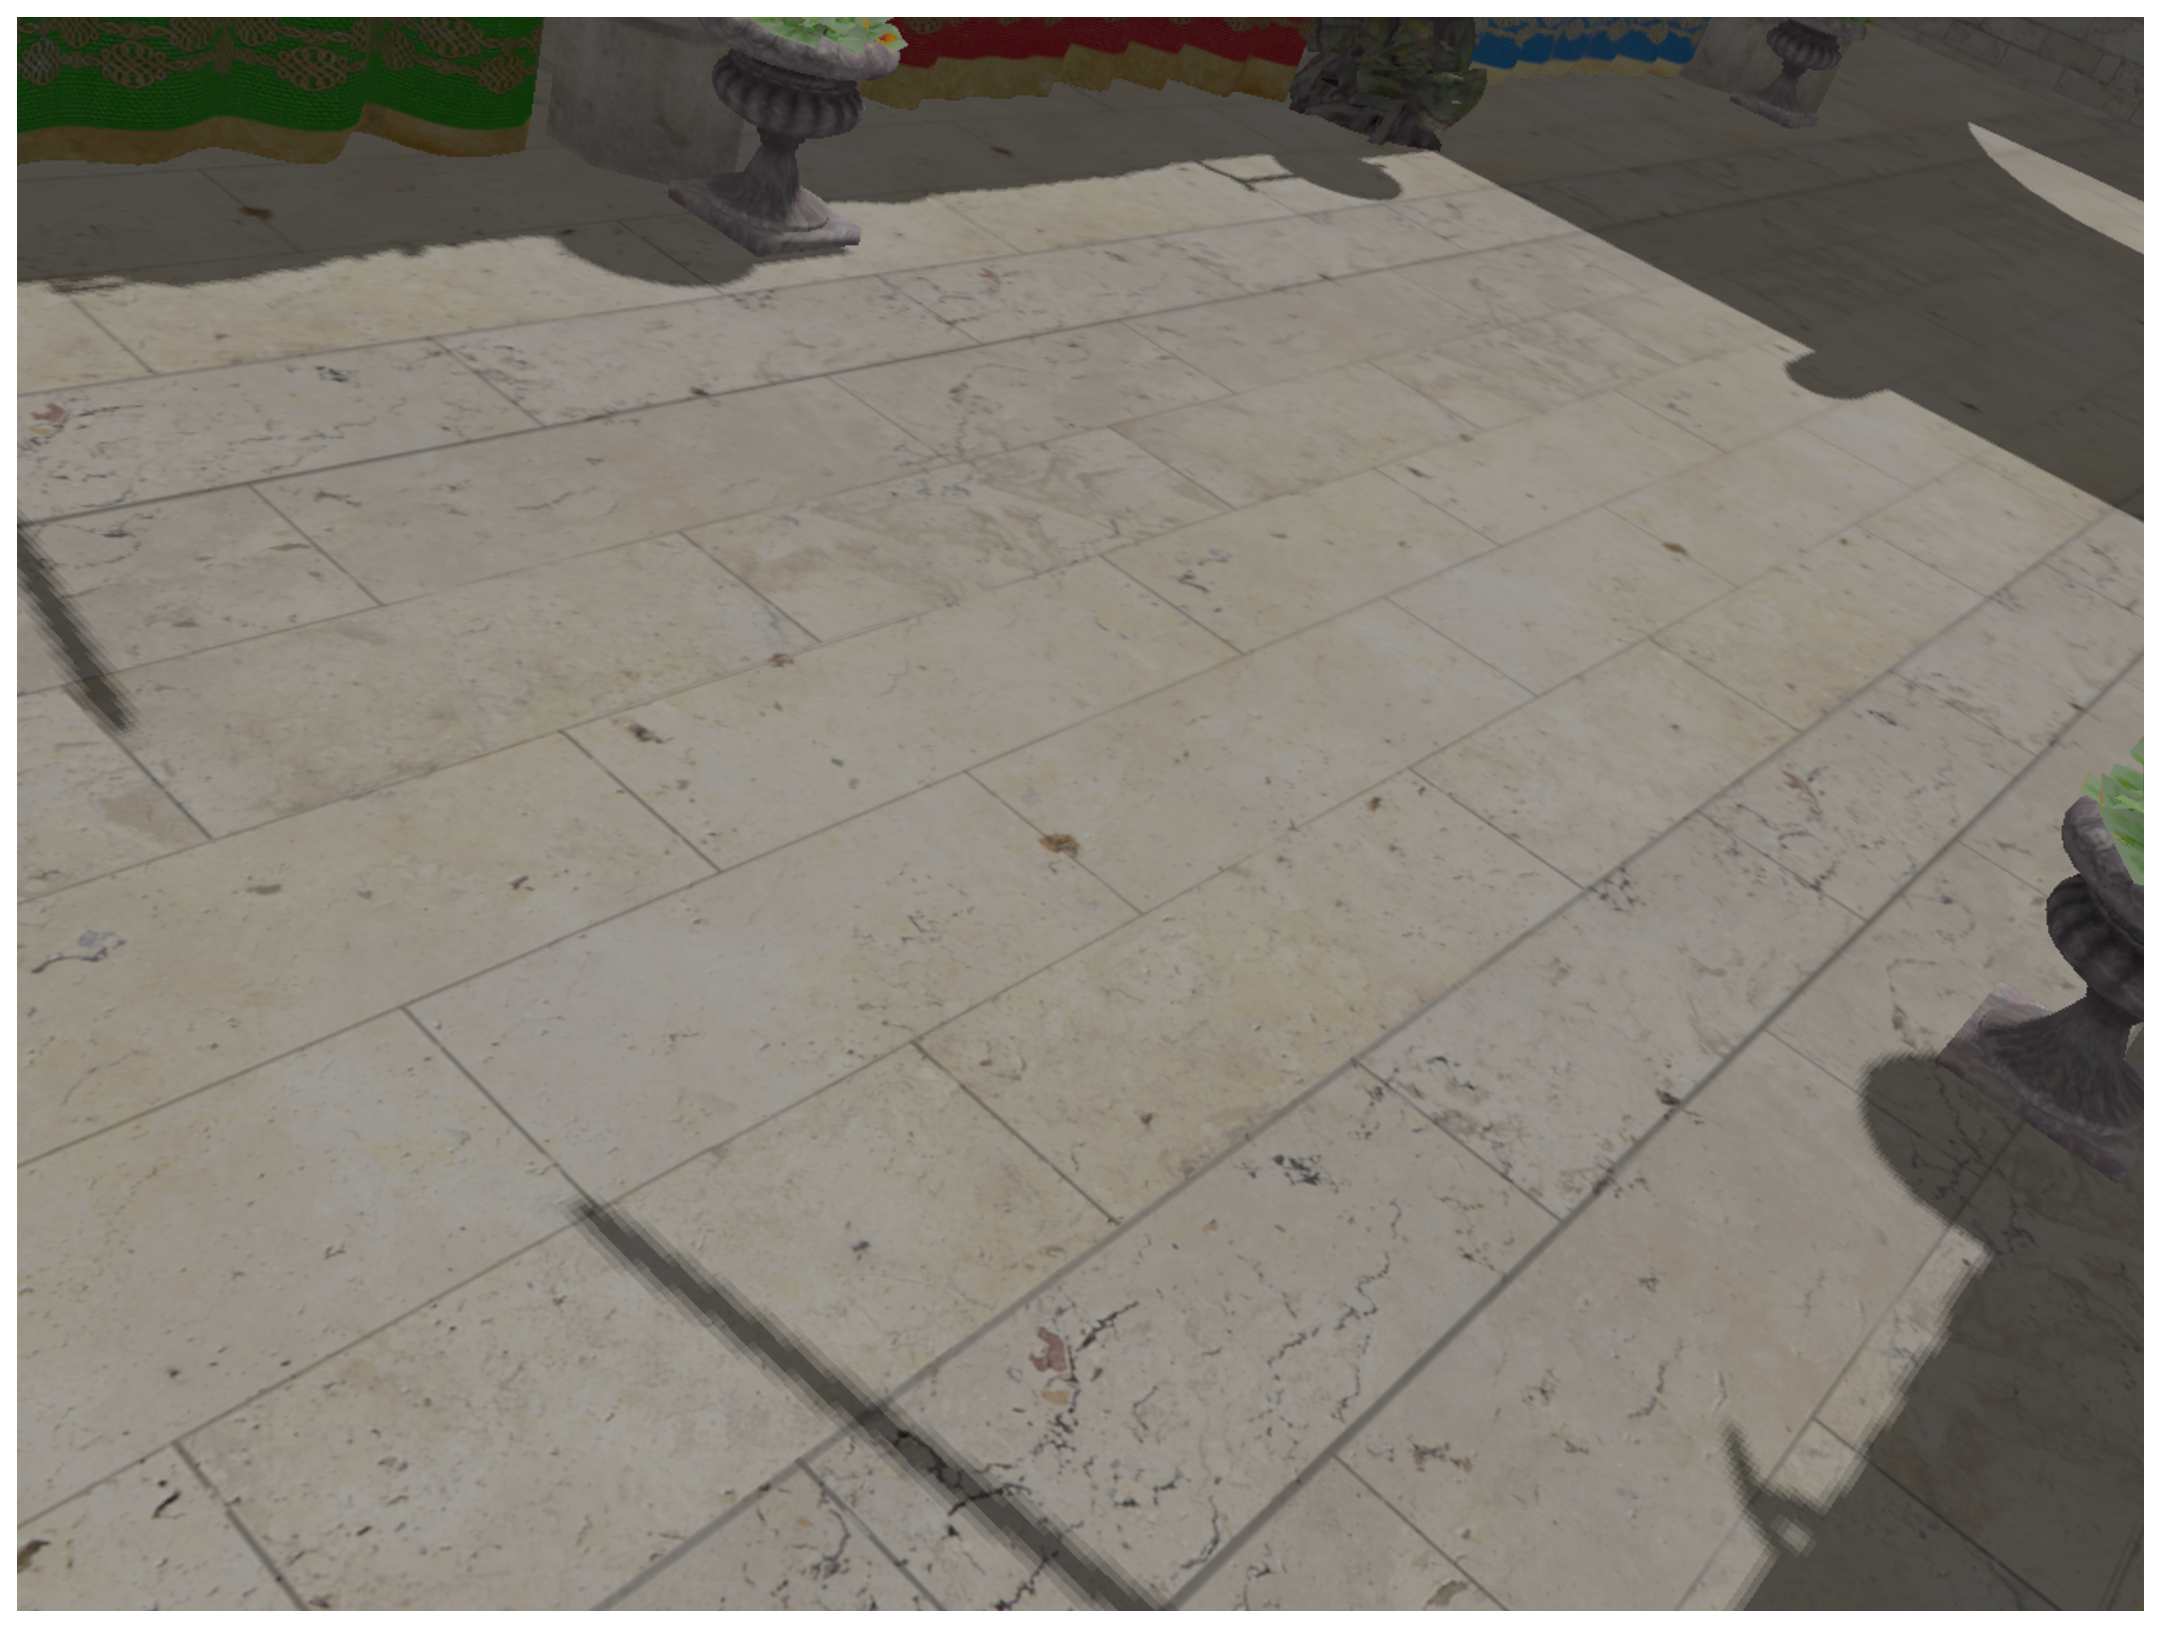
\includegraphics[width=\textwidth]{pics/shadows/shadowMapping/pcf_nearest.eps}
\end{frame}

\begin{frame}
    \frametitle{Princip}
    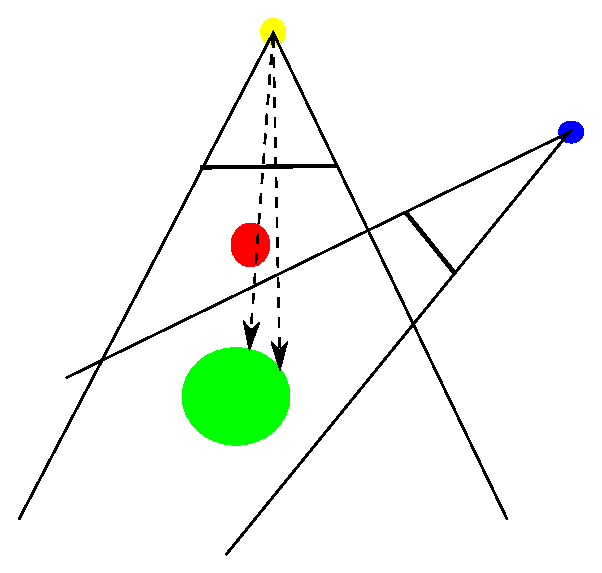
\includegraphics[height=.75\textheight]{pics/shadows/shadowMapping/smap.eps}
    \begin{itemize}
        \item Připravíme si z-buffer kamery ve světle.
        \item Porovnáváme hloubky vykreslovaných fragmentù.
    \end{itemize}
\end{frame}

\begin{frame}
    \frametitle{Hloubková mapa}
    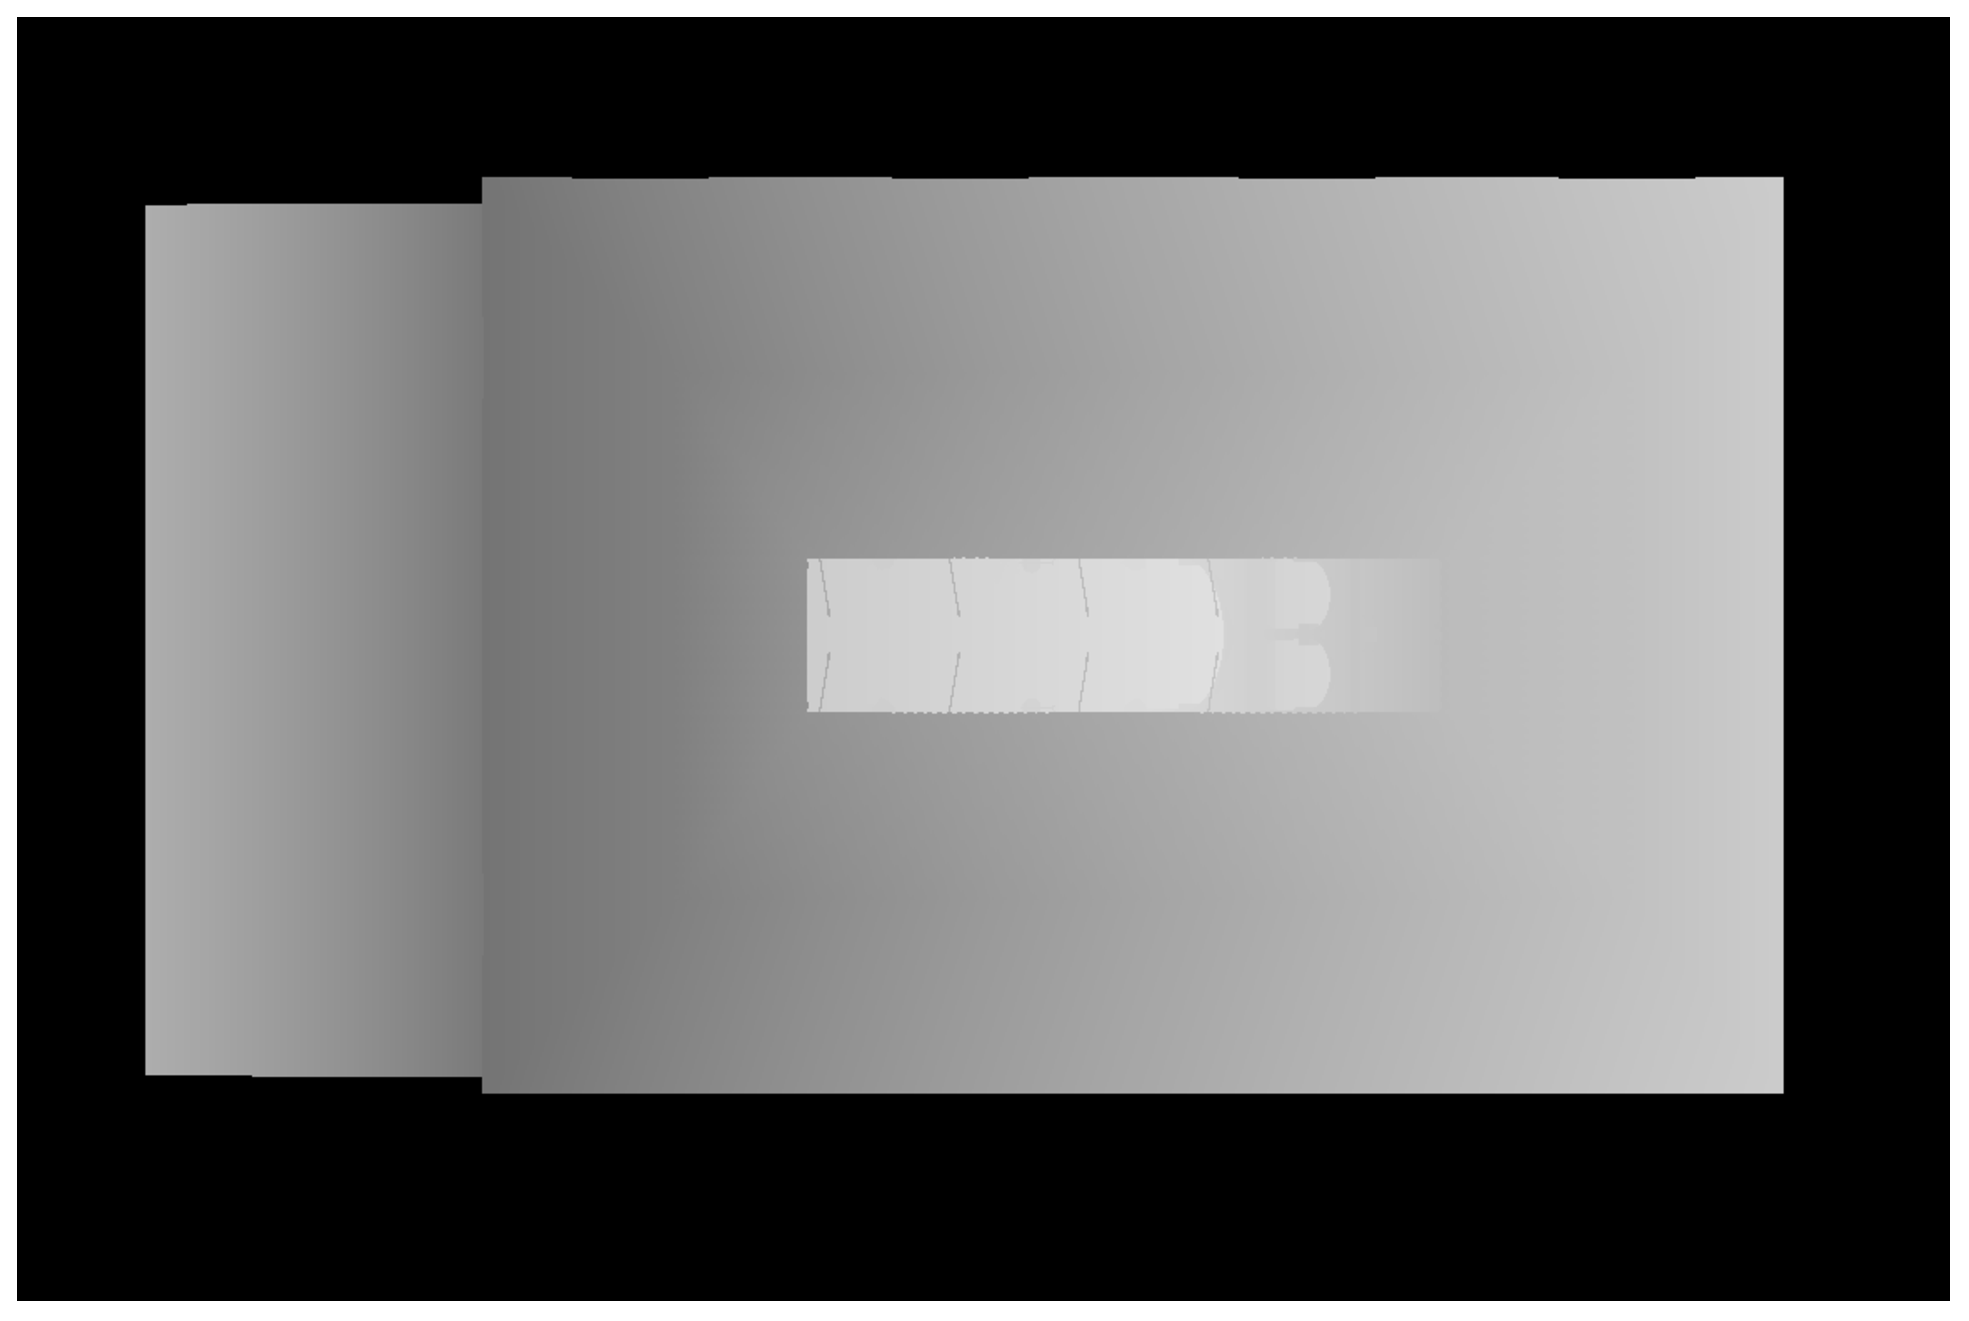
\includegraphics[width=\textwidth]{pics/shadows/shadowMapping/depth.eps}
\end{frame}


\begin{frame}
    \frametitle{Matika stínových těles}

    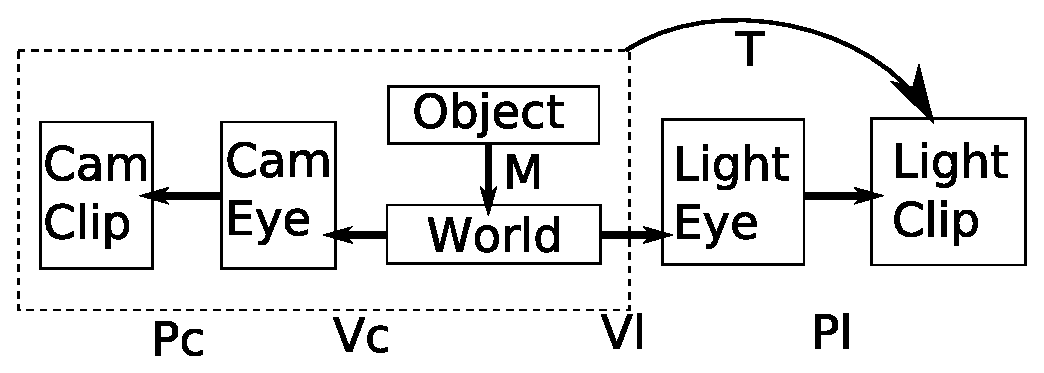
\includegraphics[width=4in]{pics/shadows/shadowMapping/smspc.eps}
    
    \vfill

    $\displaystyle T = \left( \begin{array}{cccc}
        0.5 & 0   & 0   & 0.5 \\
        0   & 0.5 & 0   & 0.5 \\
        0   & 0   & 0.5 & 0.5 \\
        0   & 0   & 0   & 1 \end{array} \right) \cdot P_l \cdot V_l \cdot M$
\end{frame}

\begin{frame}[fragile]
    \frametitle{GLSL}

{\small
  \begin{minted}[frame=lines]{glsl}
//Vertex shader
in vec4 position;
out vec4 shadowPos;
uniform mat4 shadowMat;
void main() {
    //...
    shadowPos = shadowMat*position;
    //...
}
//Fragment shader
in vec4 shadowPos;
uniform sampler2D shadow;
void main() {
    vec3 sp = shadowPos/shadowPos.w;
    if(texture(shadow, sp.xy).x < sp.z)
        gl_FragColor = shadowed_color;
    else
        gl_FragColor = unshadowed_color;
}
  \end{minted}
}
\end{frame}

\begin{frame}
    \frametitle{Shadow Acne}
    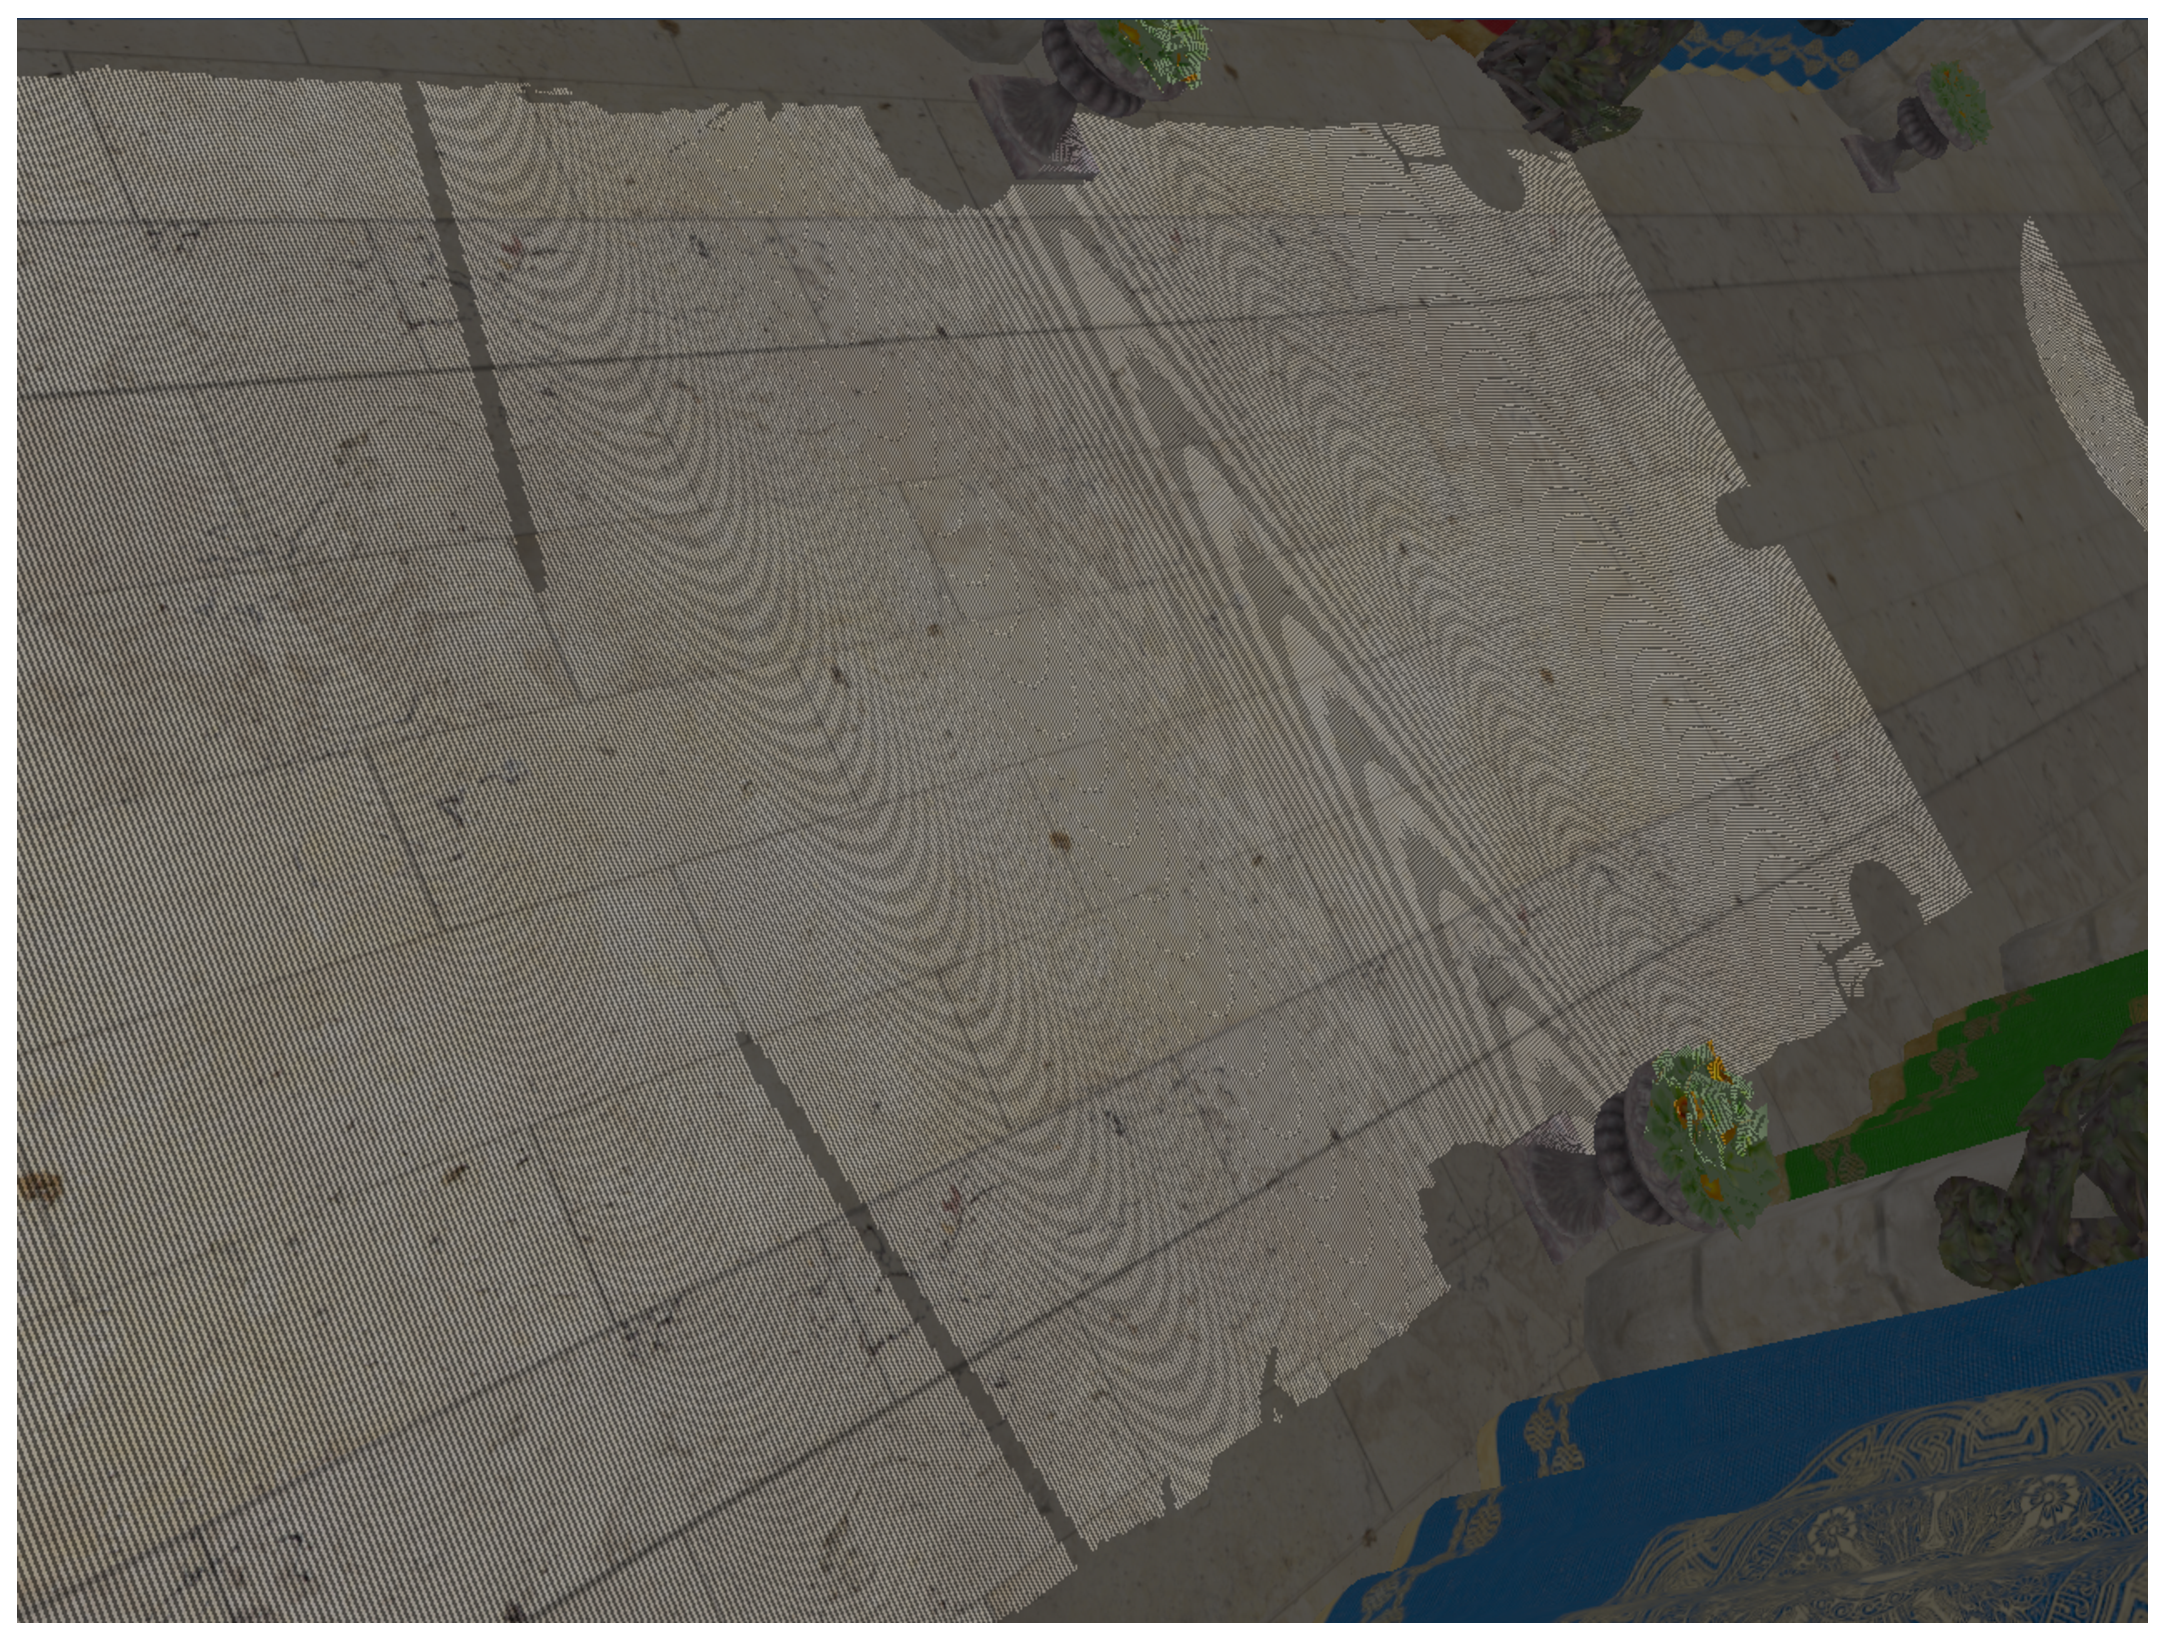
\includegraphics[width=\textwidth]{pics/shadows/shadowMapping/acne.eps}
\end{frame}

\begin{frame}[fragile]
    \frametitle{Bias}
    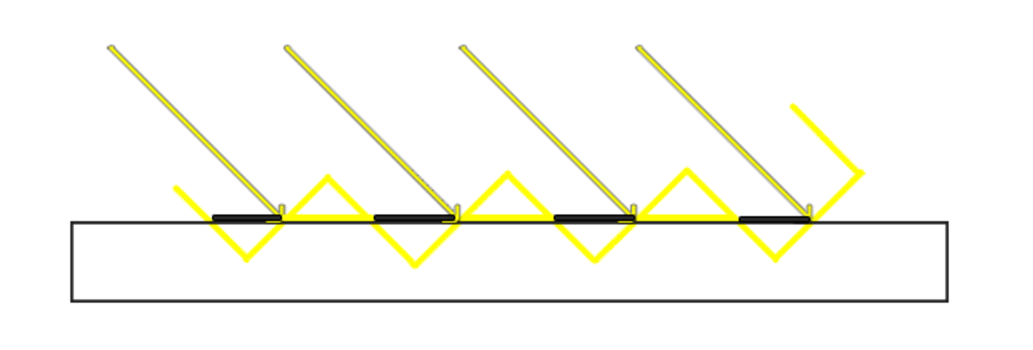
\includegraphics[width=.5\textwidth]{pics/shadows/shadowMapping/acne_before.eps}
    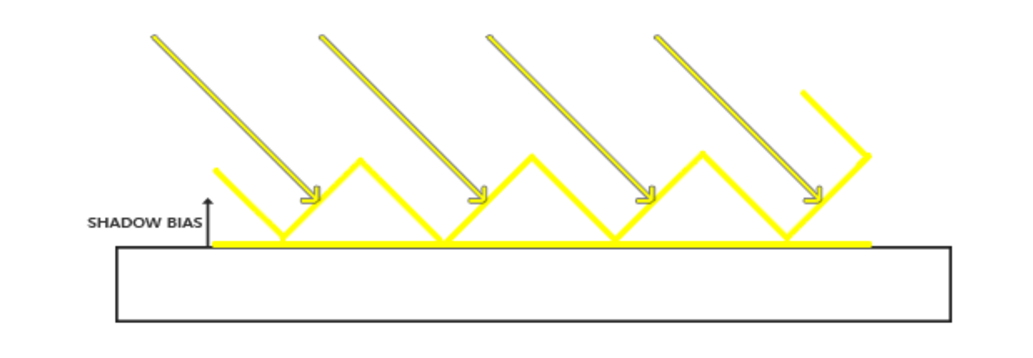
\includegraphics[width=.5\textwidth]{pics/shadows/shadowMapping/acne_after.eps}
    \vfill

{\small
  \begin{minted}[frame=lines]{glsl}
float depth = texture(shadowTexture, shadow_pos.xy).x;
float bias = max(0.05 * (1.0 - dot(N, L)), 0.005);
float shadow = shadow_pos.z - bias > depth ? 1.0 : 0.0; 
  \end{minted}
}
\end{frame}

\begin{frame}
    \frametitle{Alias}
    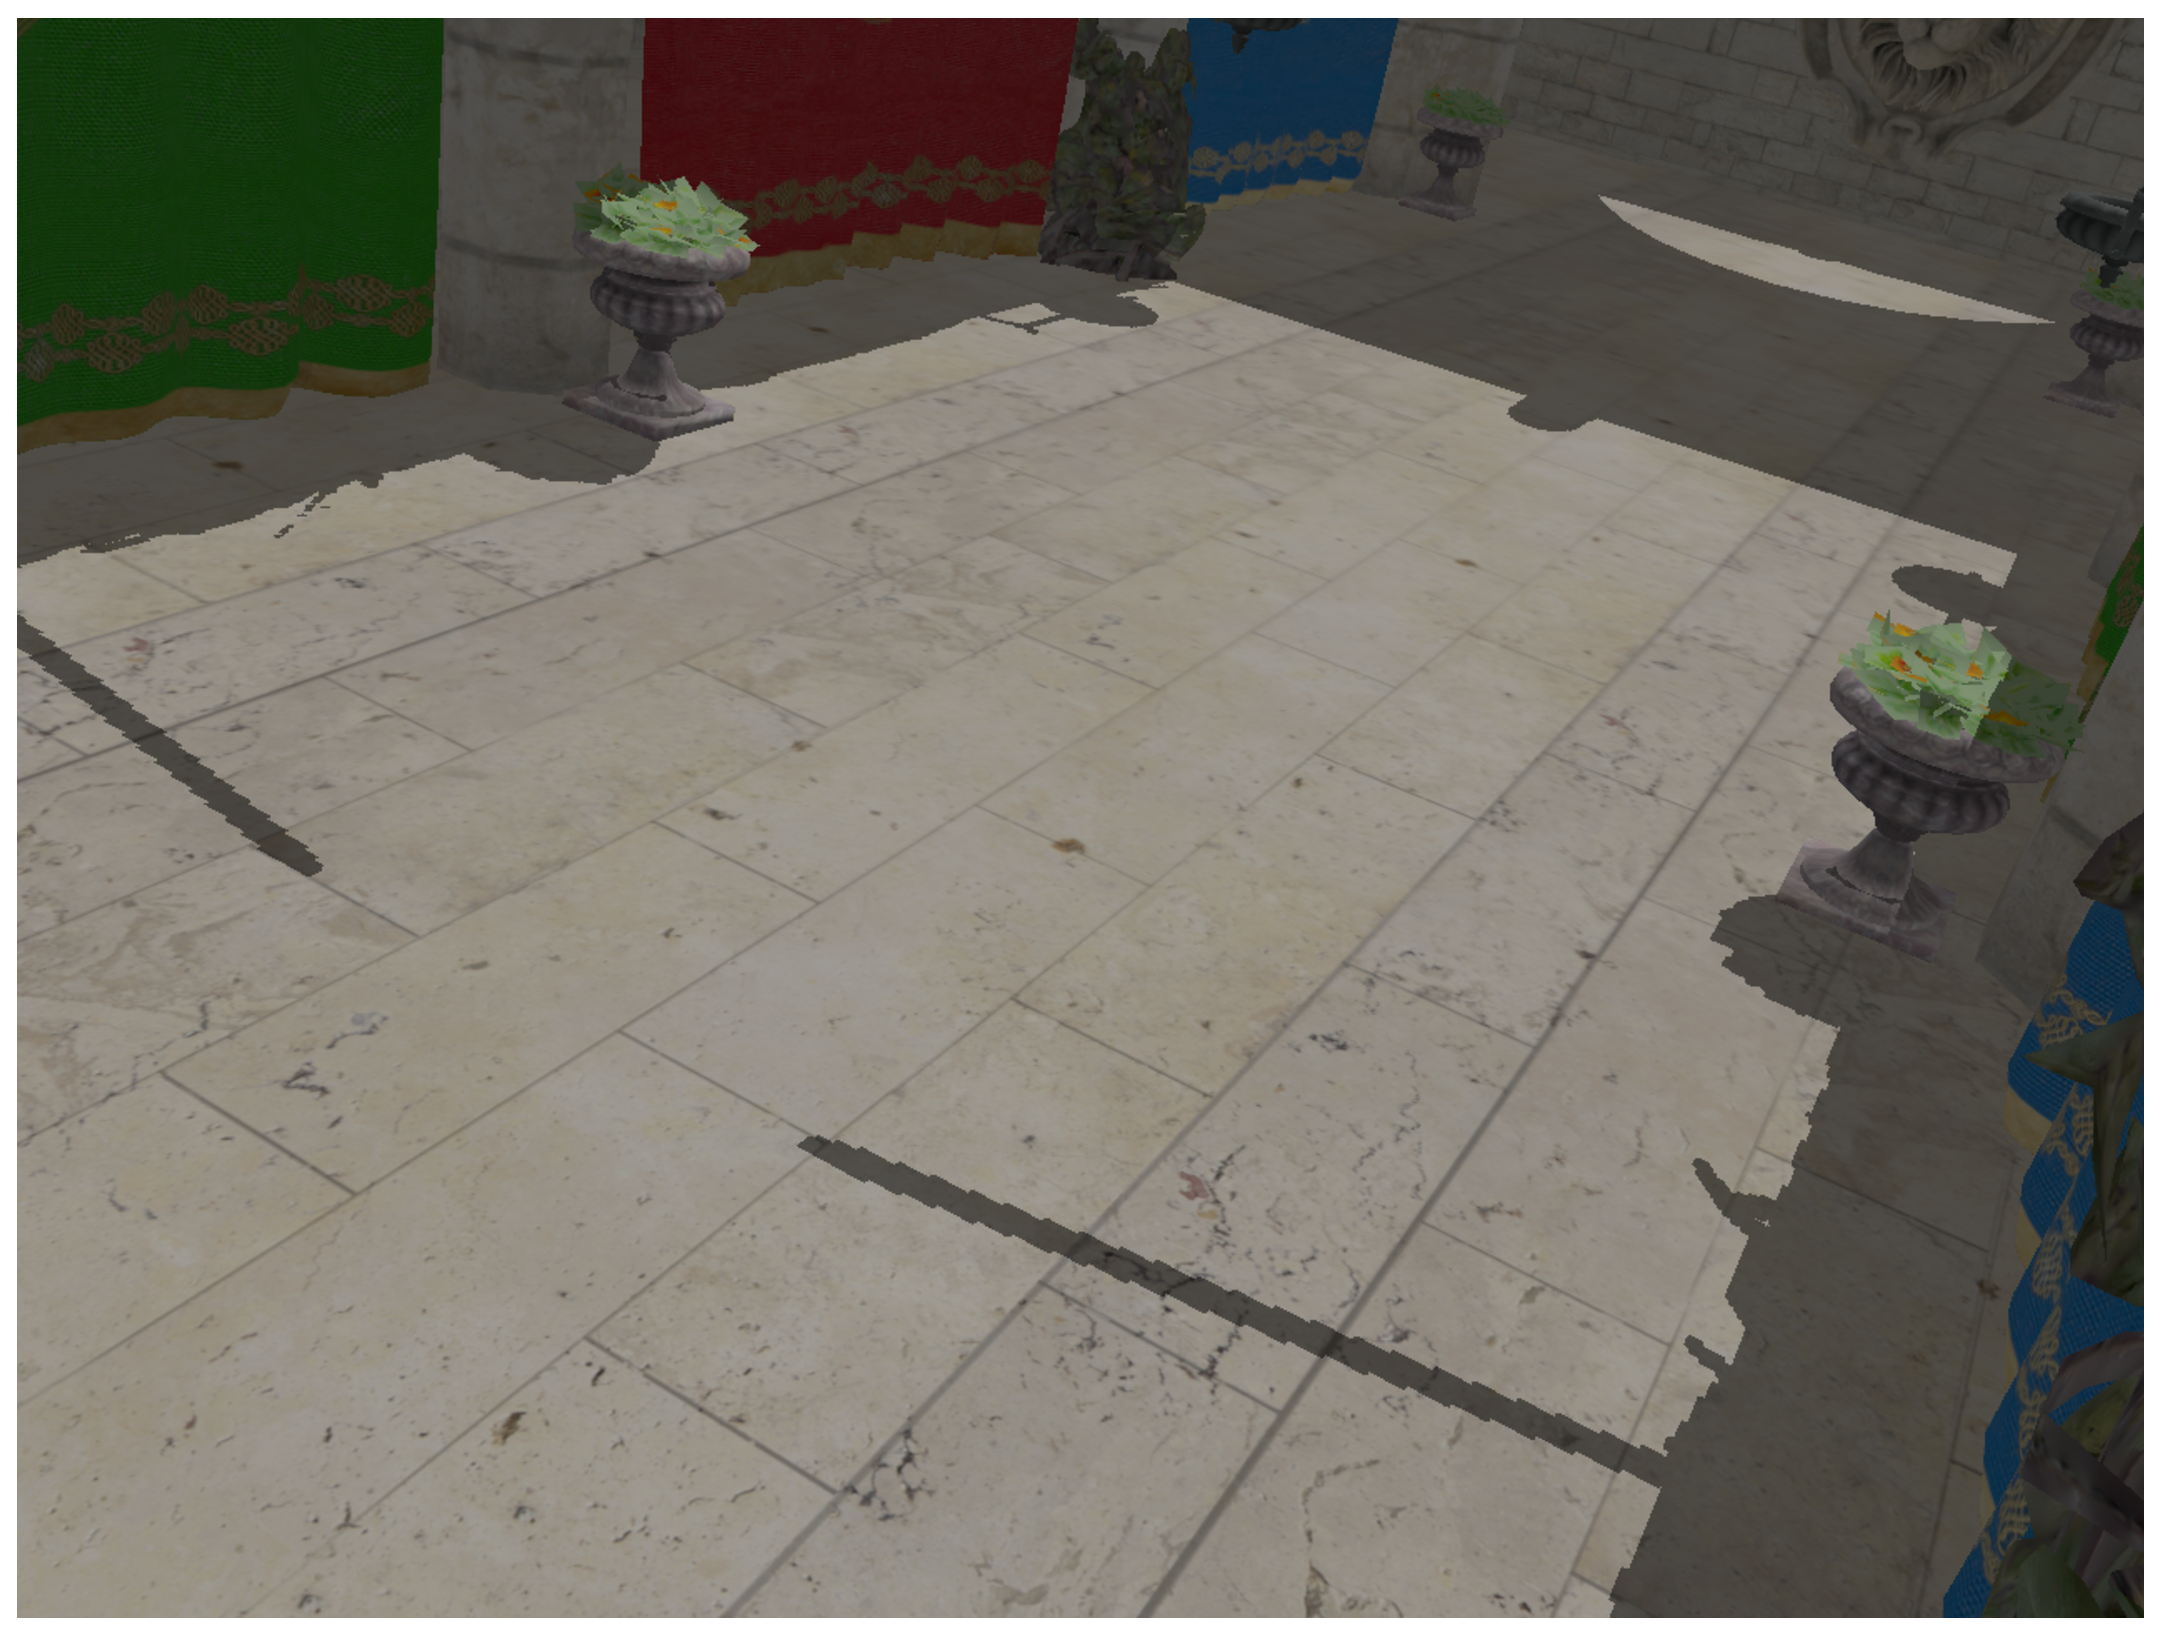
\includegraphics[width=\textwidth]{pics/shadows/shadowMapping/shadow_alias.eps}
\end{frame}

\begin{frame}
  \frametitle{Shadow-Mapping - Problems}
  \begin{itemize}
    \item Mnoho shadow-samples je nadužíváno.
    \item Mnoho shadow-samples není vůbec využito.
    \item $\to$ Zubaté hrany.
    \item Pro odstranění artefaktů je mnoho metod založeno na dělení prostoru nebo warpingu prostoru.
  \end{itemize}
  \begin{picture}(320,250)
    \put(-20,85){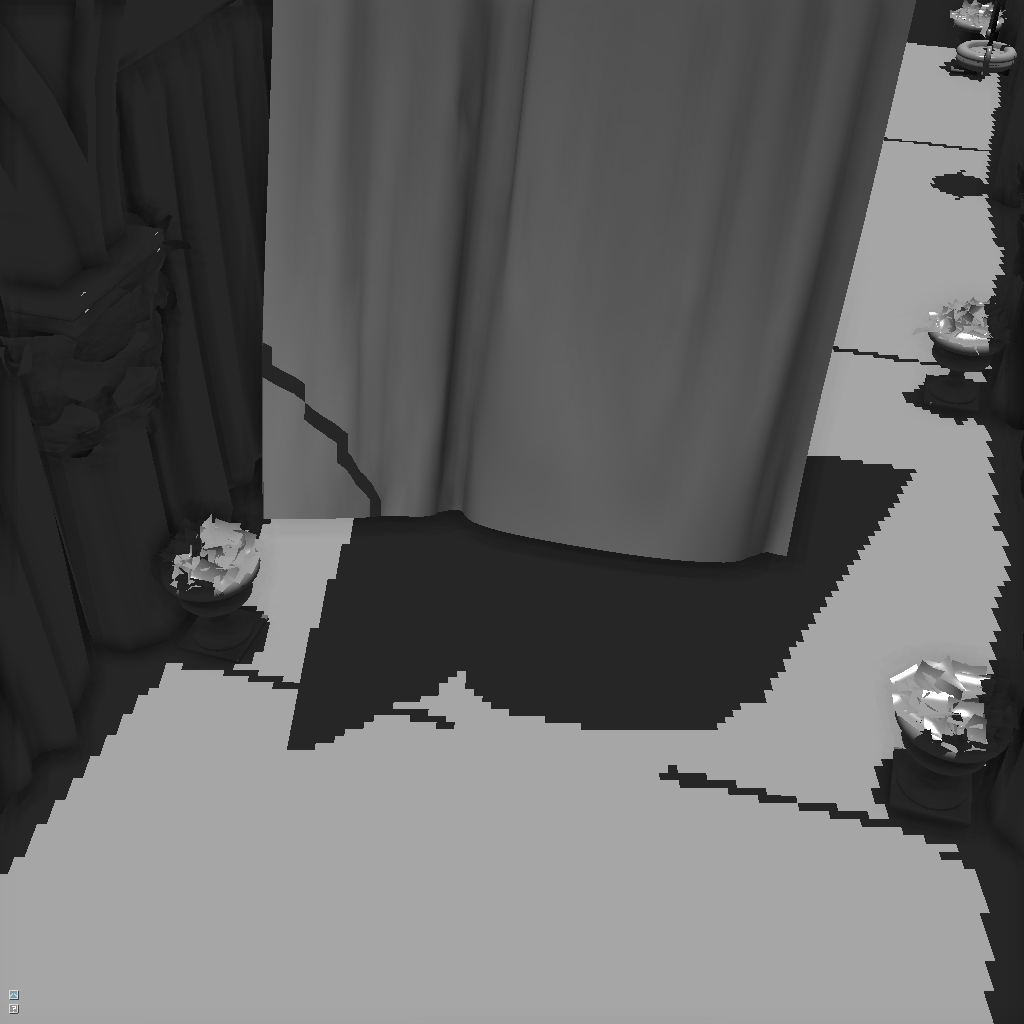
\includegraphics[height=5.5cm,keepaspectratio]{pics/shadows/shadowMapping/sponza_sm}}
    \put(160,85){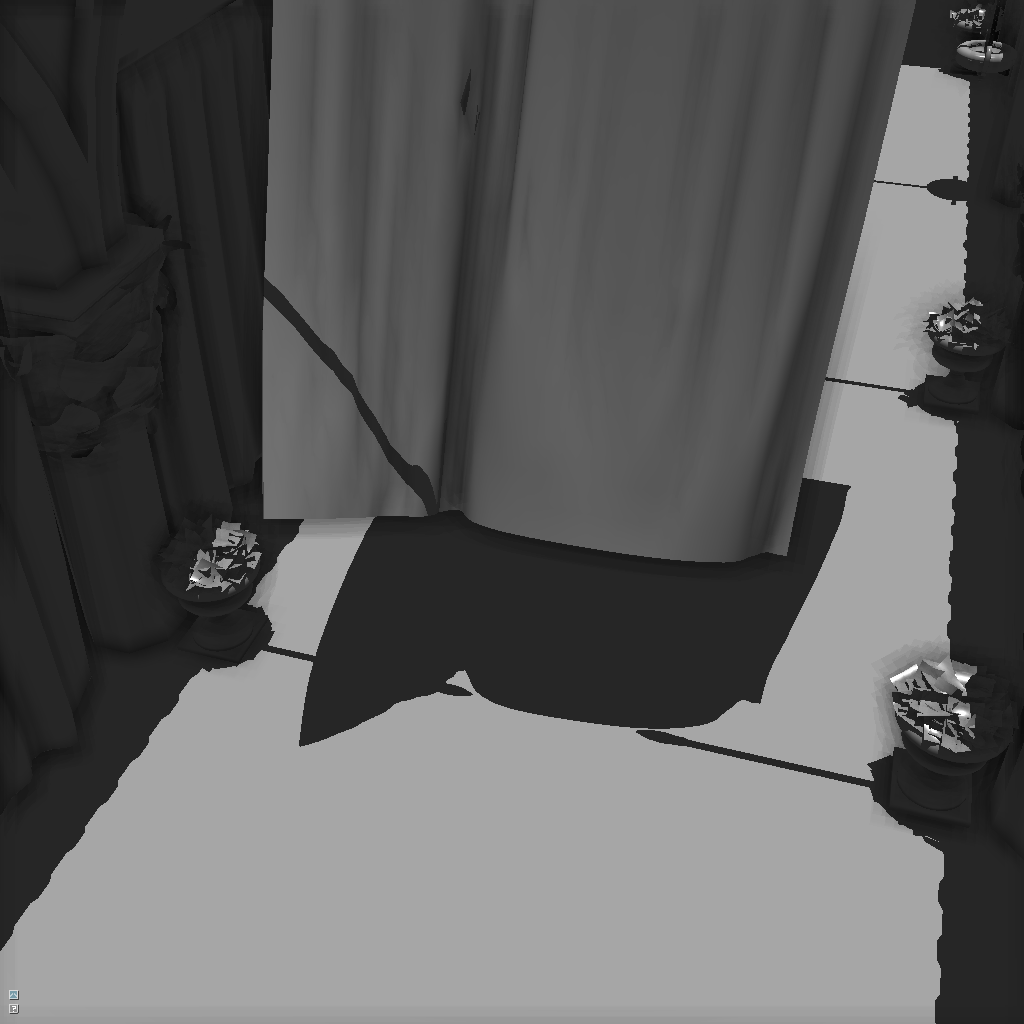
\includegraphics[height=5.5cm,keepaspectratio]{pics/shadows/shadowMapping/sponza_sv}}
  \end{picture}
\end{frame}

\begin{frame}
  \frametitle{Zubaté hrany}
  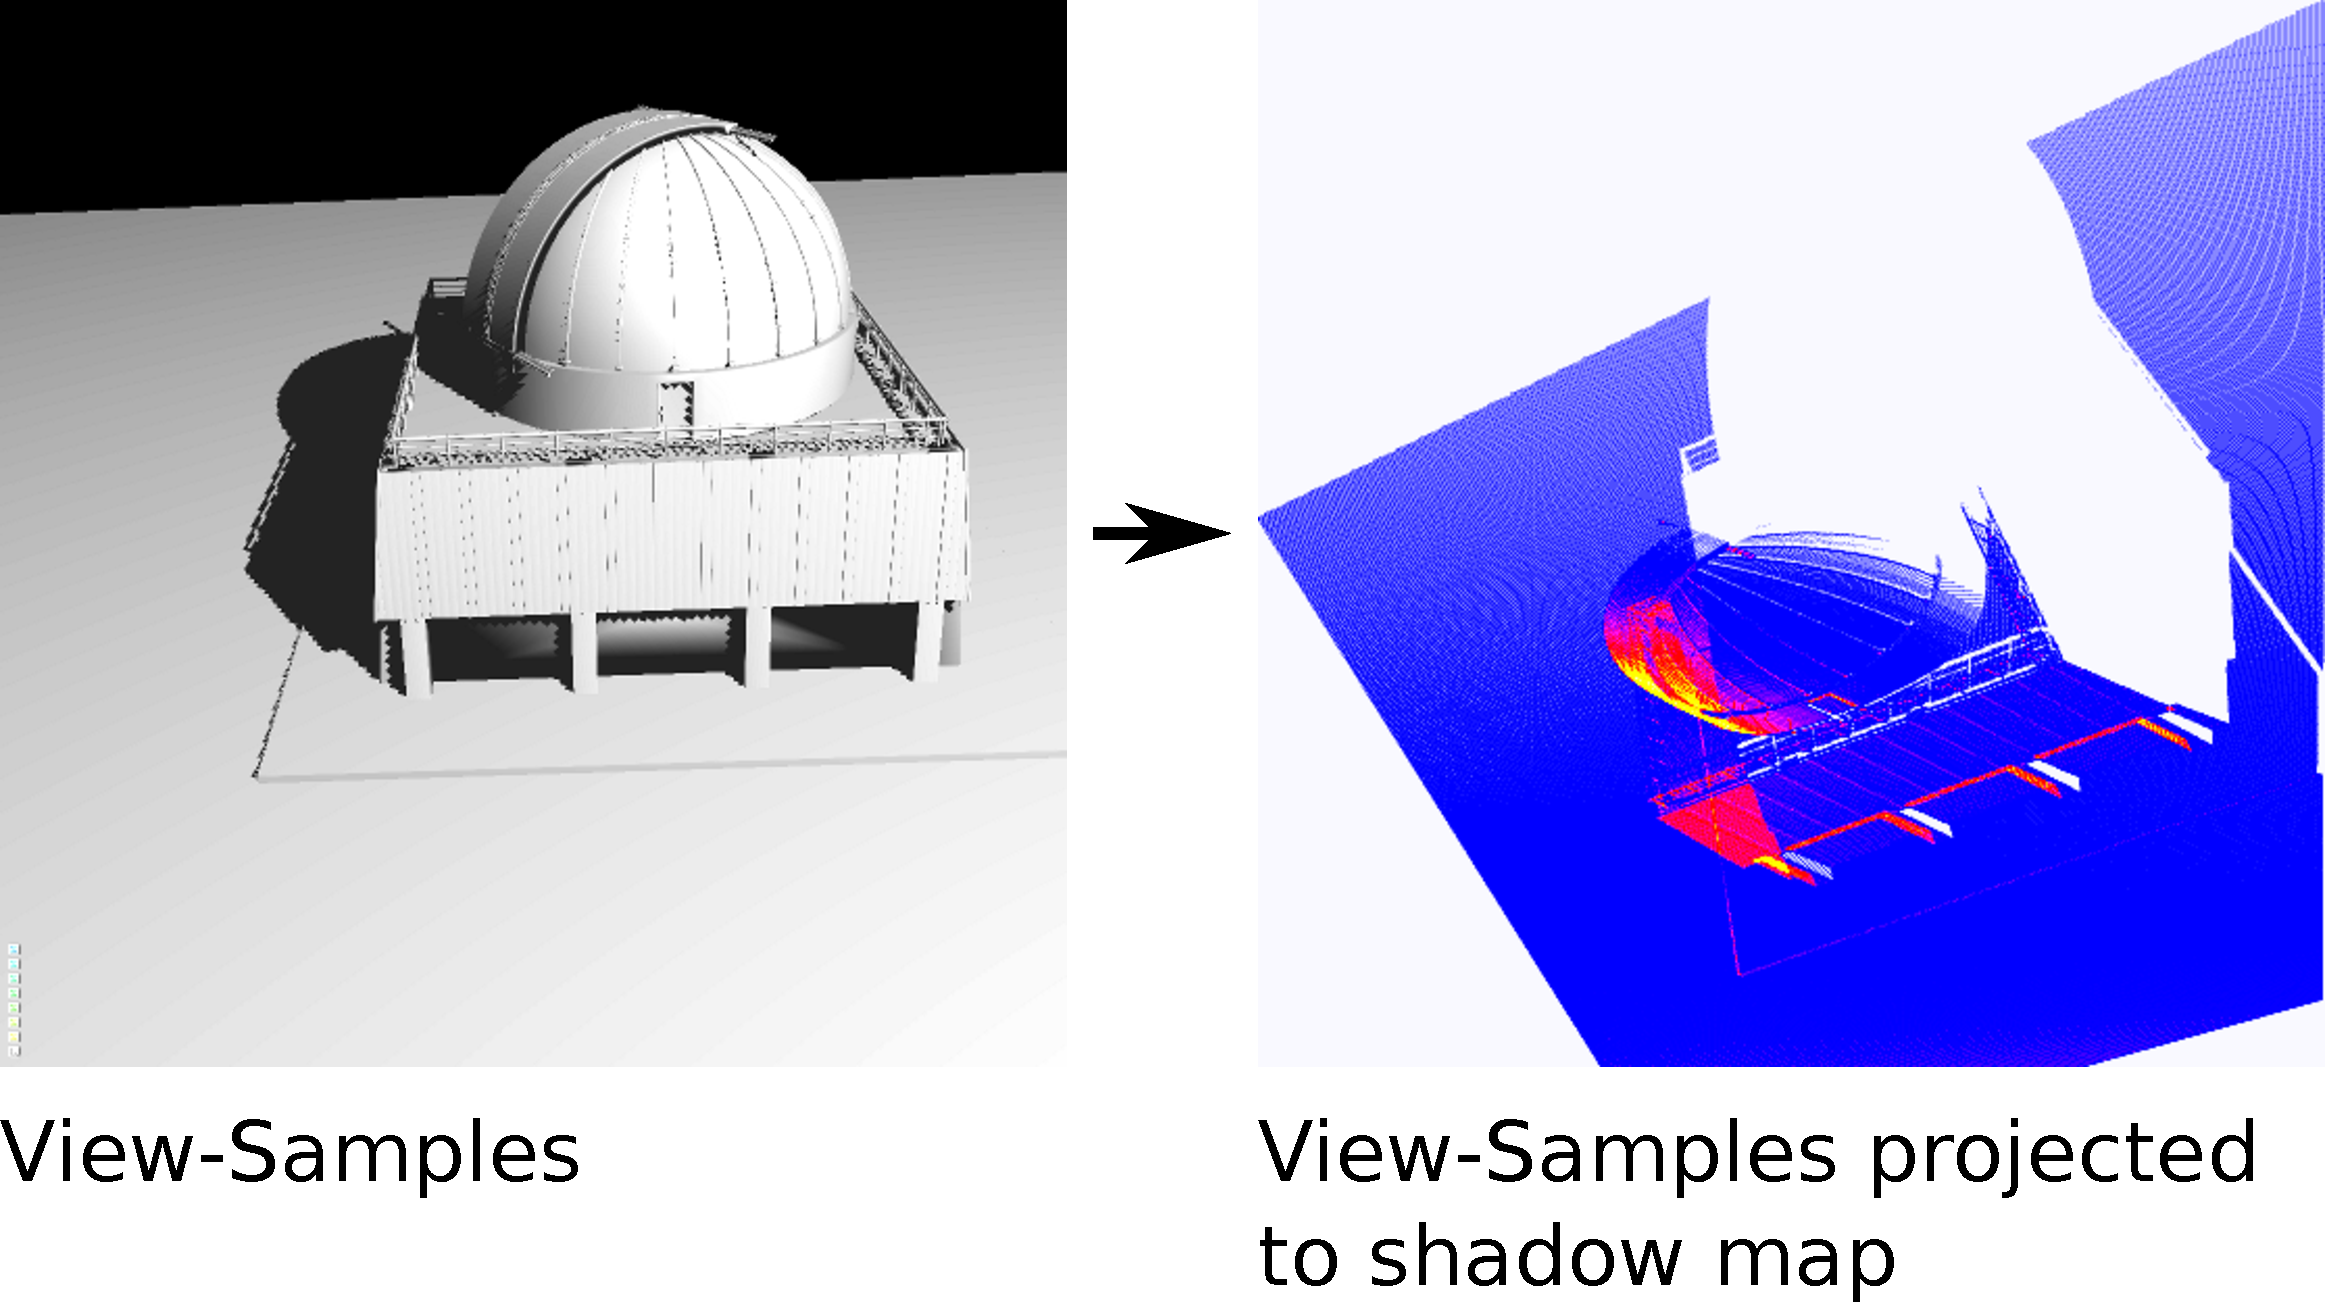
\includegraphics[width=\textwidth]{pics/shadows/shadowMapping/projectedShadowSamples}
\end{frame}

\begin{frame}
    \frametitle{Měkké stíny}
    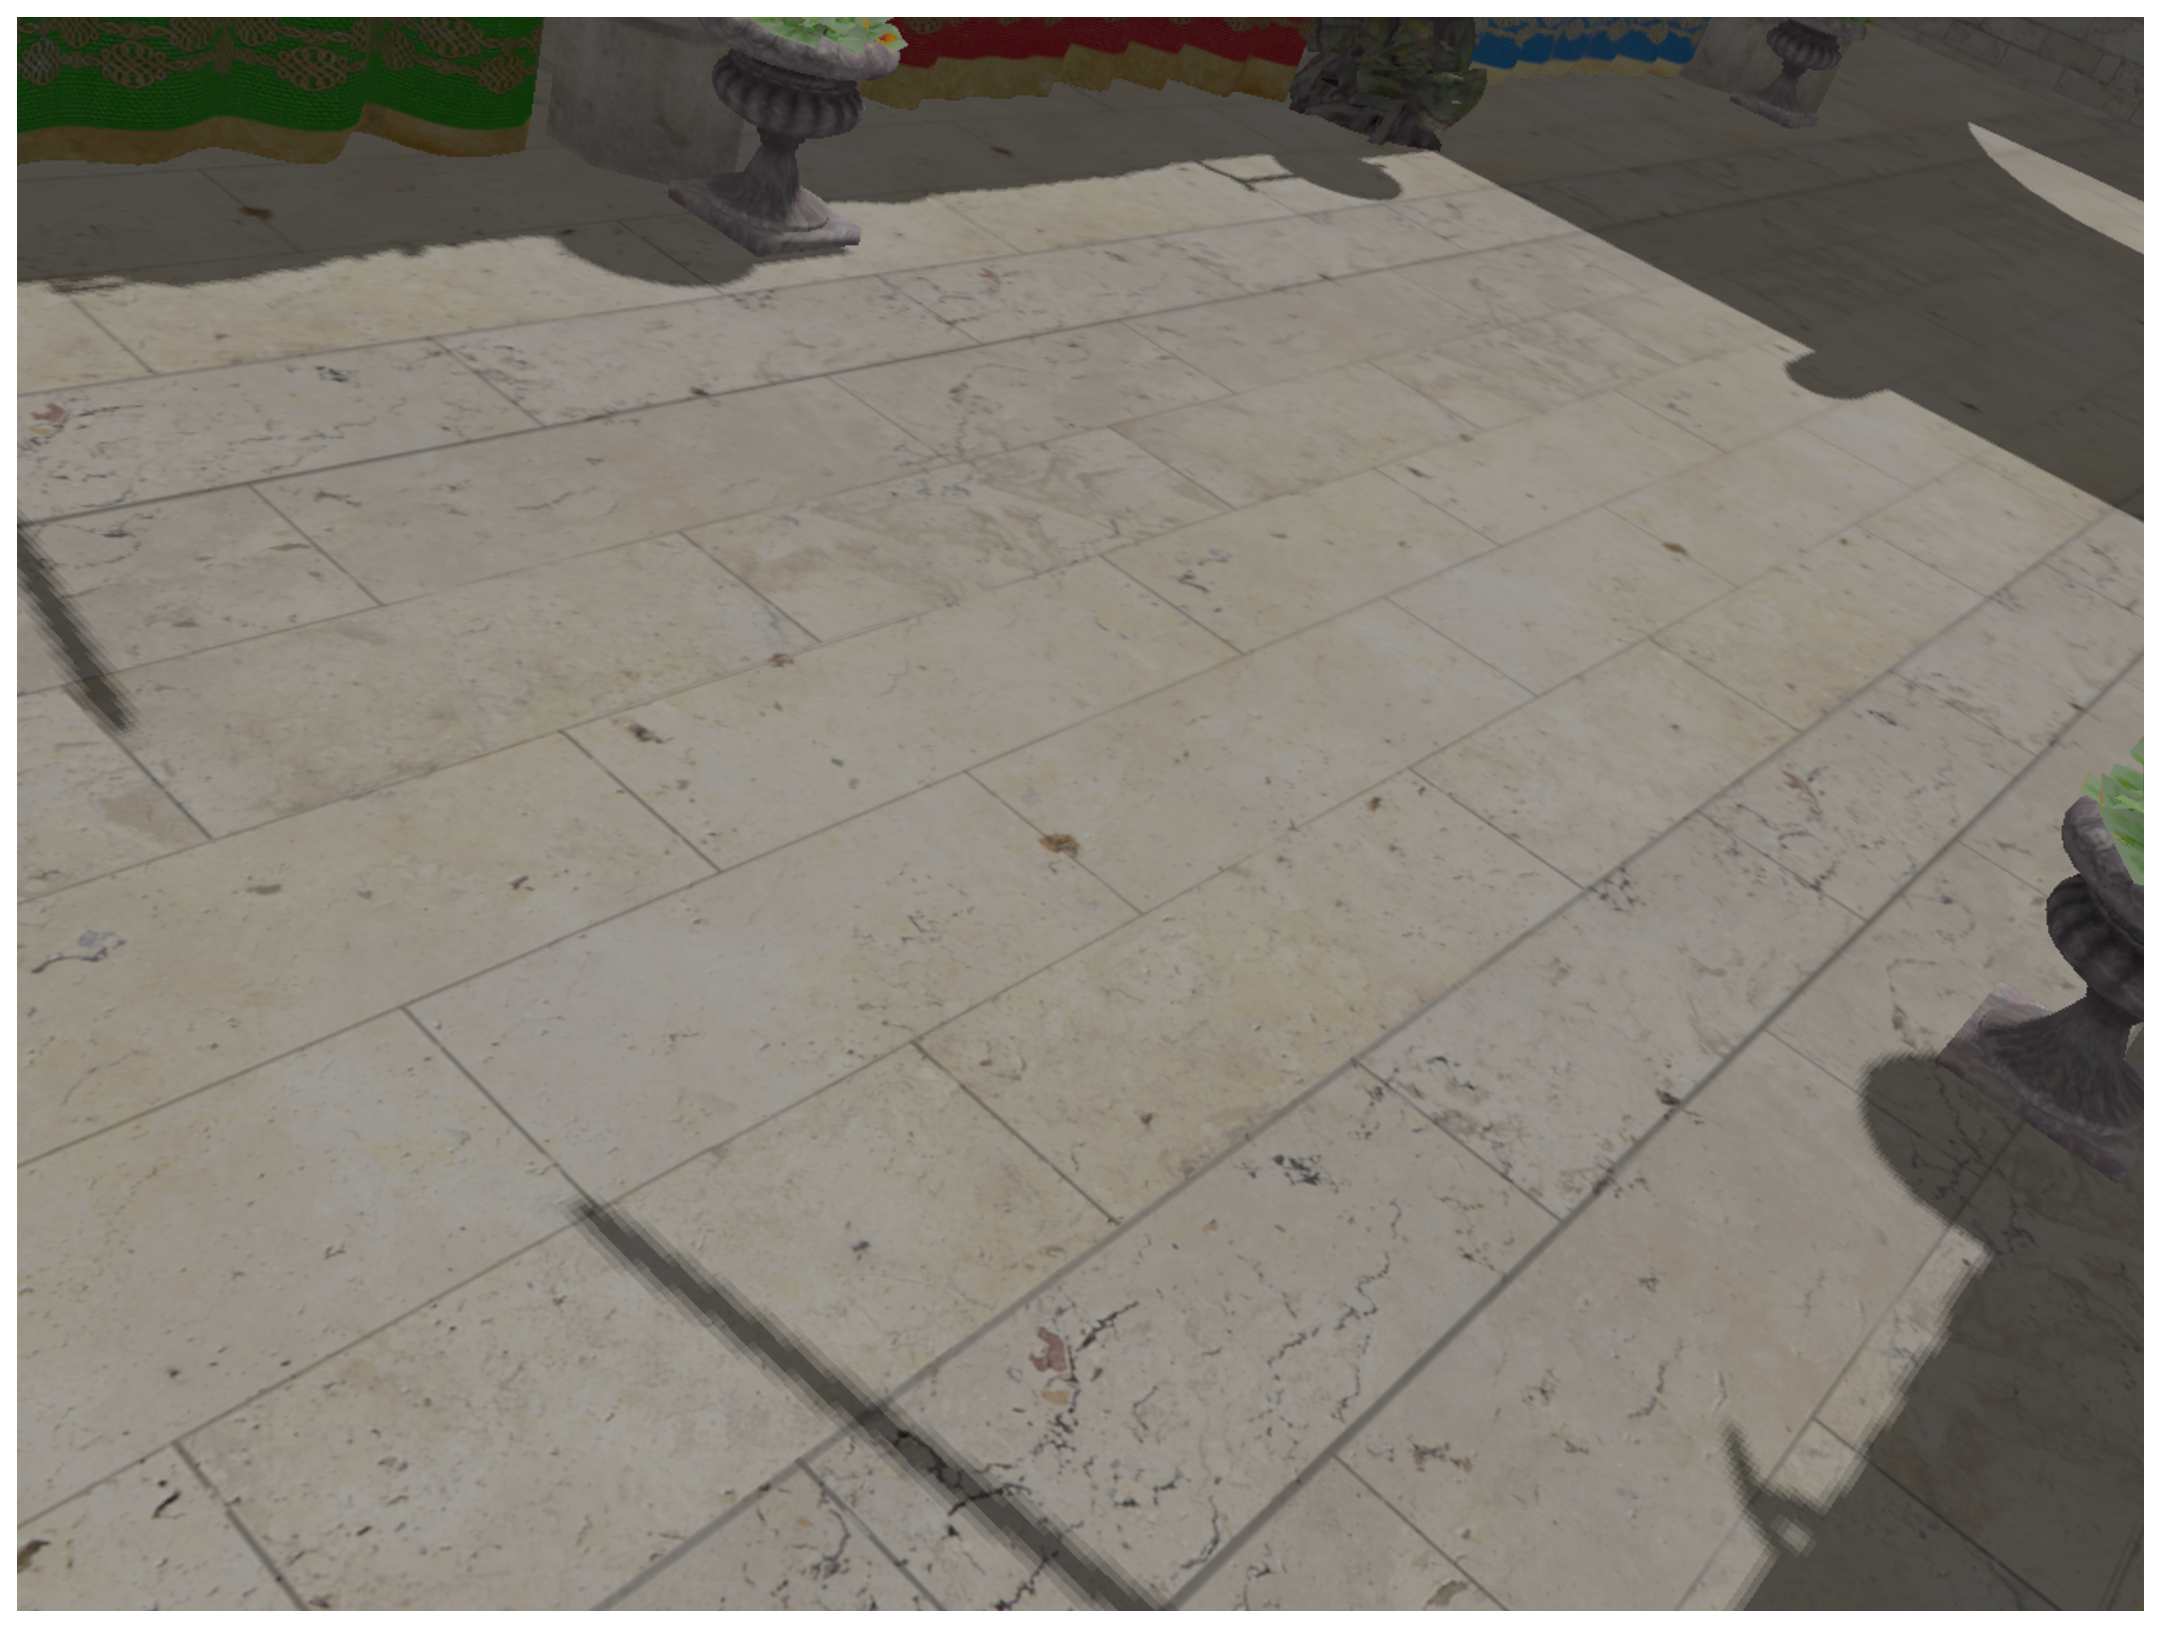
\includegraphics[width=\textwidth]{pics/shadows/shadowMapping/pcf_nearest.eps}
\end{frame}

\begin{frame}[fragile]
\frametitle{PCF}
{\small
  \begin{minted}[frame=lines]{glsl}
float shadow = 0.0;
vec2 texelSize = 1.0 / textureSize(shadowTexture, 0);
for(int x = -1; x <= 1; ++x)
{
    for(int y = -1; y <= 1; ++y)
    {
        float depth = texture(shadowTexture, 
          shadow_pos.xy + vec2(x, y) * texelSize).r; 
        shadow += shadow_pos.z - bias > depth ? 1.0 : 0.0;        
    }    
}
shadow /= 9.0;

  \end{minted}
}
\end{frame}

\begin{frame}
    \frametitle{Souhrn}
    $+$
    \begin{itemize}
        \item Rychlé
        \item Jednoduché
        \item Žádná nová geometrie
        \item Umí měkké stíny
    \end{itemize}
    \vfill
    $-$
    \begin{itemize}
        \item Všesměrová světla
        \item Omezené rozlišení textur
        \item Alias
    \end{itemize}
\end{frame}

\setbeamercolor{background canvas}{bg=fitblue}
\begin{frame}
  \frametitle{Procedurální generování}
  \begin{center}
    \Huge {\color{white}Procedurální generování}
  \end{center}
\end{frame}
\setbeamercolor{background canvas}{bg=white}

\begin{frame}
\frametitle{Procedurální generování}
	\begin{itemize}
	\item{Neukládáme data grafických objektů.}
	\item{Neukládáme vrcholy, pixely, barvy, ...}
	\item{Ukládáme šablony a způsob vygenerování grafického objektu.}
	\item{Uložení algoritmu pro vygenerování zabírá pár kB.}
	\item{Uložení v textovém souboru - parametry.}
	\item{Můžeme generovat i šablony.}
	\item{Málo místa pro uložení vs doba generování.}
	\end{itemize}
\end{frame}

\begin{frame}
\frametitle{Fraktály}
	\begin{figure}[h]
		
\includegraphics[width=10cm,keepaspectratio]{pics/procedural/fractal.jpg}
	\end{figure}
\end{frame}

\begin{frame}
\frametitle{Fraktály}
	\begin{figure}[h]
		
\includegraphics[width=2.8cm,keepaspectratio]{pics/procedural/weed0.jpg}
		
\includegraphics[width=2.8cm,keepaspectratio]{pics/procedural/weed1.jpg}
		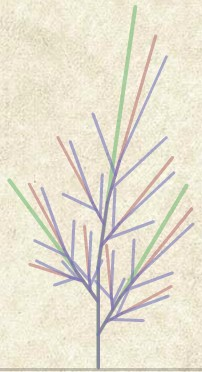
\includegraphics[width=2.8cm,keepaspectratio]{pics/procedural/weed2.jpg}
		
\includegraphics[width=2.8cm,keepaspectratio]{pics/procedural/weed3.jpg}
	\end{figure}
	\url{http://www.dangries.com/Flash/FractalMakerExp/FractalMaker_exp.html}
\end{frame}

\begin{frame}
\frametitle{L-systém}
	\begin{figure}[h]
		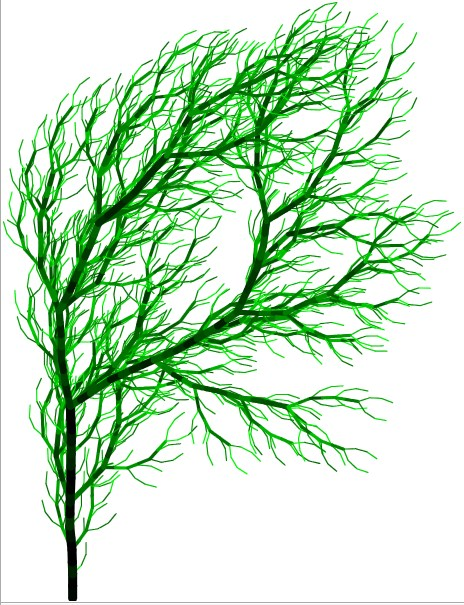
\includegraphics[width=4cm,keepaspectratio]{pics/procedural/lsystem.jpg}
		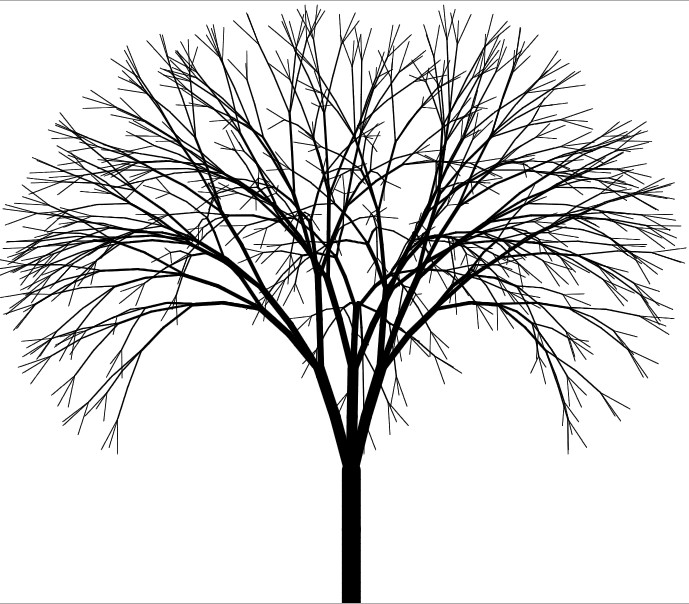
\includegraphics[width=4cm,keepaspectratio]{pics/procedural/lsystem1.jpg}
	\end{figure}
	\url{http://malsys.cz/}
\end{frame}

\begin{frame}
\frametitle{L-systém}
	\begin{figure}[h]
		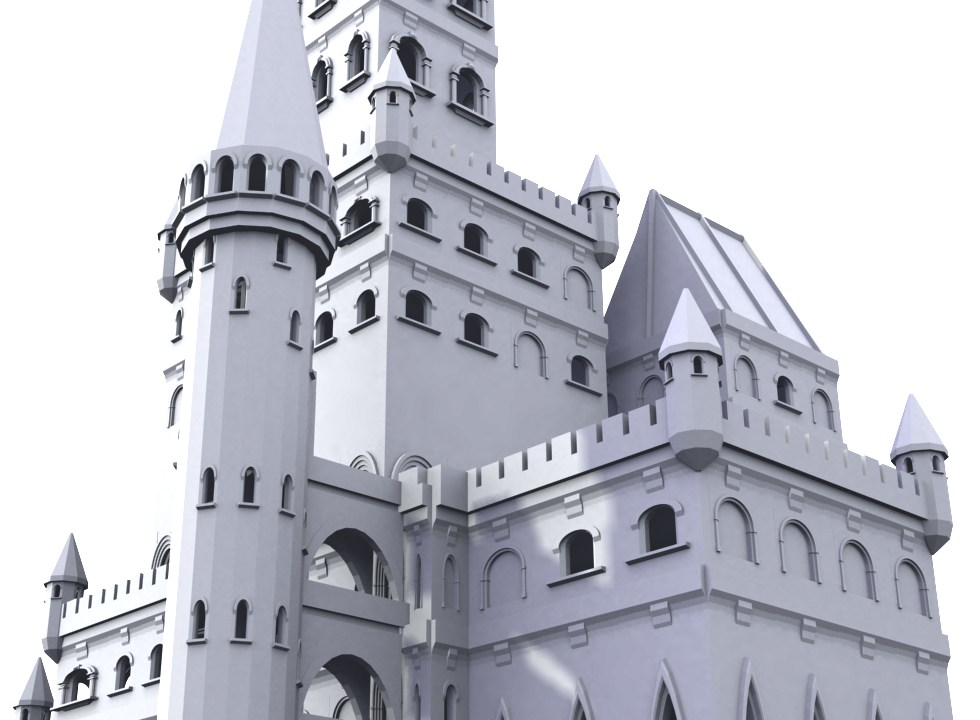
\includegraphics[width=10cm,keepaspectratio]{pics/procedural/castle.jpg}
	\end{figure}
	\url{http://procworld.blogspot.com/}
\end{frame}

\begin{frame}
\frametitle{Šumy a voroného diagramy}
	\begin{itemize}
		\item Perlin/Simple noise
    \item Voroného diagramy
	\end{itemize}
	\begin{figure}[h]
		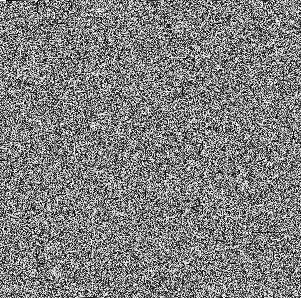
\includegraphics[width=3cm,keepaspectratio]{pics/procedural/simple_noise}
		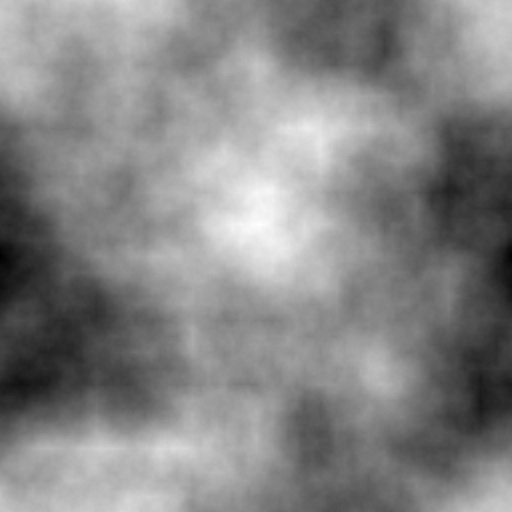
\includegraphics[width=3cm,keepaspectratio]{pics/procedural/midpoint_noise}
		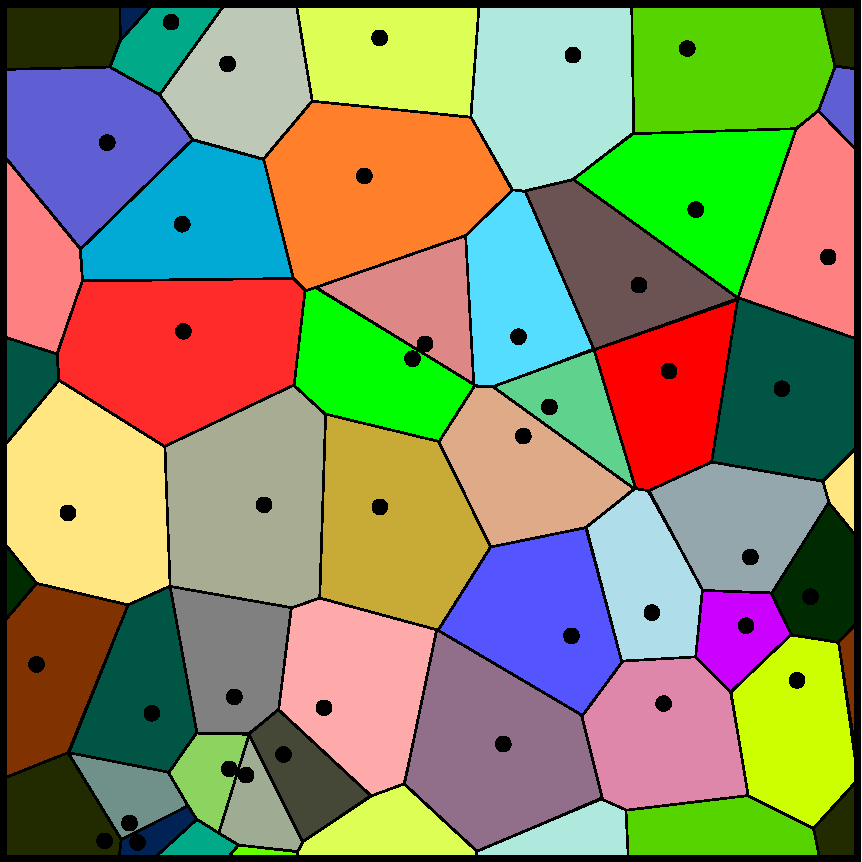
\includegraphics[width=3cm,keepaspectratio]{pics/procedural/voronoid}
	\end{figure}
\end{frame}


\begin{frame}
\frametitle{Textury založené na šumech}
	\begin{figure}[h]
		
\includegraphics[width=3cm,keepaspectratio]{pics/procedural/tex00.jpg}
		\includegraphics[width=3cm,keepaspectratio]{pics/procedural/tex01.jpg}
		\includegraphics[width=3cm,keepaspectratio]{pics/procedural/tex02.jpg}
	\end{figure}
\end{frame}

\begin{frame}
    \frametitle{Procedurální textury}

    \begin{columns}[c]
    \column{.5\textwidth}
        \includegraphics[width=\textwidth]{pics/procedural/vase.eps}
    \column{.5\textwidth}
        \begin{itemize}
            \item Výpočet hodnoty v shaderu.
            \item Málo paměti.
            \item Neomezené rozlišení.
            \item Vhodné pro dema.
            \item Šum
        \end{itemize}
    \end{columns}
\end{frame}

\begin{frame}
    \frametitle{Šum v grafice}
    Chceme šumové funkce
    \begin{itemize}
        \item float noise(float p)
        \item float noise(vec2 p)
        \item ...
    \end{itemize}
    \vfill
    \begin{itemize}
        \item Pseudonáhodné
        \item Výstup v $[0,1]$ nebo $[-1,1]$
        \item Deterministické
        \item Omezené frekvenční spektrum
    \end{itemize}
\end{frame}

\begin{frame}[fragile]
    \frametitle{Hodnotový šum}
    \begin{columns}[c]
    \column{.5\textwidth}
        \begin{itemize}
            \item Náhodně vygenerovaná textura.
            \item Rychle se opakuje.
            \item Interpolaci a opakování zařídí OpenGL.
        \end{itemize}
    \column{.5\textwidth}
        \includegraphics[width=\textwidth]{pics/procedural/value_noise.eps}
    \end{columns}

  \begin{minted}[frame=lines]{glsl}
float noise(vec2 p)
{
    return 2*texture(noiseTexture, p).x - 1;
}
  \end{minted}
\end{frame}

\begin{frame}[fragile]
    \frametitle{Gradientní šum}
    \begin{columns}[c]
    \column{.5\textwidth}
        \begin{itemize}
            \item V textuře jsou \textbf{gradienty}.
            \item Spočítáme si směrové vektory od \textbf{texelů} ke \textbf{vzorku}.
            \item Skalární součin směrů s gradienty dává výsledný šum.
        \end{itemize}
        \includegraphics[width=.5\textwidth]{pics/procedural/grad_noise.eps}
    \column{.5\textwidth}
        \includegraphics[width=\textwidth]{pics/procedural/perlin_noise.eps}
    \end{columns}
    Perlin K.; Implementing Improved Perlin Noise, GPU Gems\\
    Green S.; Implementing Improved Perlin Noise, GPU Gems 2
\end{frame}

\begin{frame}[fragile]
    \frametitle{Fraktální šum}
    \begin{columns}[c]
    \column{.5\textwidth}
        \begin{itemize}
            \item Sčítáme vrstvy o různé frekvenci a amplitudě
            \item Oktávy
        \end{itemize}
    \column{.5\textwidth}
        \includegraphics[width=\textwidth]{pics/procedural/1dnoise-fractal.eps}
    \end{columns}
  \begin{minted}[frame=lines]{glsl}
float fnoise(vec2 p)
{
    return noise(p)
        + 0.5*noise(2*p)
        + 0.25*noise(4*p);
}
  \end{minted}
\end{frame}

\begin{frame}
    \frametitle{Výsledek}
    \includegraphics[width=\textwidth]{pics/procedural/2dnoise-fractal.eps}
\end{frame}

\begin{frame}
    \frametitle{Jednoduchý priklad}
    \includegraphics[width=\textwidth]{pics/procedural/drevo.eps}
\end{frame}
 
\begin{frame}[fragile]
    \frametitle{Letokruhy}
    \includegraphics[width=.5\textwidth]{pics/procedural/letokruhy.eps}

  \begin{minted}[frame=lines]{glsl}
float d = length(model_pos.xy);
float t = mod(d*10, 1);
  \end{minted}
\end{frame}

\begin{frame}[fragile]
    \frametitle{Letokruhy obarvíme}
    \includegraphics[width=.5\textwidth]{pics/procedural/letokruhy_barva.eps}

  \begin{minted}[frame=lines]{glsl}
vec3 brown = vec3(140, 90, 27)/255;
vec3 yellow = vec3(188, 140, 42)/255;

float t = smoothstep(0.2, 0.4, mod(length(model_pos.xy)*10, 1));
vec3 color = (1-t)*brown + t*yellow;
  \end{minted}
\end{frame}

\begin{frame}[fragile]
    \frametitle{Přidáme šum}
    \includegraphics[width=.6\textwidth]{pics/procedural/drevo.eps}

  \begin{minted}[frame=lines]{glsl}
vec2 noisy_pos = model_pos.xy
    + 0.1*fnoise(model_pos.xy);

float t = smoothstep(0.2, 0.4, mod(length(noisy_pos)*10, 1));
vec3 color = (1-t)*brown + t*yellow;
  \end{minted}
\end{frame}


%\begin{frame}
  \frametitle{References}
  \begin{itemize}
    \item \url{http://www.opengl.org/sdk/docs/}
    \item \url{http://www.opengl.org/documentation/glsl/}
    \item \url{http://www.opengl.org/registry/}
  \end{itemize}
\end{frame}



\bluepage{Thank you for your attention! \vspace{10 mm} Questions?}

\end{document}
